\section{与先前工作的扩展比较}
\subsection{KV 缓存优化}
\label{appendx: kv opt}
\paragraph{多层KV 缓存管理。}
为了缓解GPU 显存压力，Pensieve等系统~\citep{Yu_2025}，Continuum~\cite{li2025continuumefficientrobustmultiturn}，Strata~\citep{xie2025stratahierarchicalcontextcaching}、以及ShadowKV~\citep{sun2025shadowkvkvcacheshadows} 利用硬件内存层次结构，包括 GPU HBM、CPU DRAM 和 NVMe SSD 进行 KV 缓存管理。这些分层缓存机制通过将不活动的 KV 状态卸载到较低层存储并在请求恢复时将它们预取回 GPU 来减轻瞬时抢占。然而，这些方法的实际效率从根本上受到设备和主机存储器之间的层间带宽的限制。在高频智能体工作流中，频繁换入和换出周期的开销通常会抵消多层缓存的优势，如下所示 \autoref{sec:experiments}.

% \textbf{Predictive and Workflow-Aware Context Persistence.}
% To mitigate the overhead of KV-cache re-prefill, recent works’ KV cache management has shifted from reactive eviction to proactive persistence. Systems like Continuum~\citep{li2025continuumefficientrobustmultiturn} utilize temporal heuristics to predict request arrival intervals and pin active caches accordingly.

% However, these frameworks primarily target dynamic serving scenarios, prioritizing step-wise and end-to-end latency. Furthermore, their reliance on semantic tool classification fails to account for the significant intra-class variance present in remote model API calling and compilers.

\paragraph{分布式KV 缓存管理。}
智能体状态的分布式管理给 KV 缓存驱逐和抢占策略带来了极大的复杂性。而像BanaServe这样的系统~\citep{he2025banaserveunifiedkvcache} 以及LMCache~\citep{liu2025lmcacheefficientkvcache} 虽然跨 DP 节点启用 KV 缓存传输，但它们在大批量智能体服务和部署中的性能通常受到有限互连带宽的限制。智能体工作流中强大的程序内依赖性需要频繁的状态传输，而无需程序级管理，这很容易在服务或部署期间使网络饱和。

为了绕过这些带宽瓶颈，标准推理系统如 vLLM KV 感知路由器~\citep{vllm_kvaware_routing} 和 SGLang 模型网关~\citep{zheng2024sglangefficientexecutionstructured} 采用 KV 感知路由策略，根据前缀位置或会话 ID 将请求固定到特定节点。同样，Vortex~\citep{yuan2025vortexovercomingmemorycapacity} 引入会话感知预取以最小化跨节点数据传输延迟。然而，这些方法缺乏在 DP 节点之间动态迁移活动程序状态的能力。缺乏工作负载转移会导致整个集群内存利用率严重不平衡，如图所示 \autoref{fig:dp unbalance}。托管长时间运行的智能体程序的节点无法将状态卸载到空闲对等点，从而导致资源利用率碎片化和总吞吐量下降。

\subsection{KV 缓存优化的扩展实验结果}
\label{sec: pd+offload}
\paragraph{KV 缓存卸载实验。}
我们使用LMCache研究了KV 缓存卸载~\cite{liu2025lmcacheefficientkvcache} 作为解决容量限制的潜在补救措施。虽然卸载理论上可以利用 CPU 或 SSD 存储来扩展有效内存空间，但我们使用 vLLM + LMCache 的实现揭示了一个关键瓶颈：PCIe 带宽不足以维持智能体工作负载固有的高频上下文切换和大容量数据传输。如所示 \autoref{fig:lmcache}，服务GLM-4.6型号时~\cite{5team2025glm45agenticreasoningcoding} 配合mini-SWEAgent框架~\cite{yang2024sweagentagentcomputerinterfacesenable}，频繁的换入和换出操作带来的延迟损失抵消了GPU 显存容量的优势，导致在繁重的智能体工作负载下吞吐量严重下降。

\paragraph{预填充解码 (PD) 分解实验。}
我们还探索了PD分解~\cite{zhong2024distservedisaggregatingprefilldecoding}，一种聊天机器人服务的标准优化，通过将解码阶段与预填充干扰隔离开来。然而，当应用于以持续上下文增长为特征的智能体工作负载时，我们观察到 PD 分解 \textbf{\textit{加剧}} 抖动。通过将集群划分为仅预填充和仅解码节点，可用于处理预填充的有效 HBM 池明显小于统一架构中的 HBM 池。这种内存碎片会导致系统达到容量限制并在低得多的并发级别下触发抖动，如图所示 \autoref{fig:throughput_pd}。这些结果表明，通用架构优化不能替代主动管理工作集的以程序为中心的调度器。

\begin{figure}[b]
    \centering
    % --- 左边的图 ---
    % 将容器宽度设为 0.49 (占左半边空间)
    \begin{subfigure}[b]{0.49\linewidth}
        \centering
        % 图片宽度设为 0.6 (相对于容器)，实际效果约为页面的 0.3
        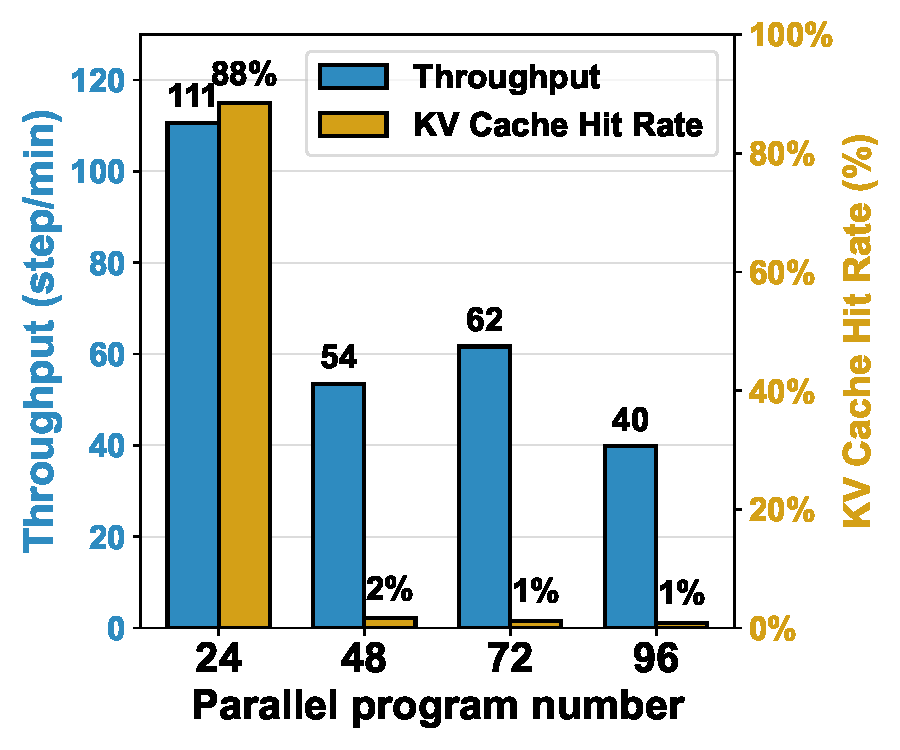
\includegraphics[width=0.99\linewidth]{Figures/lmcache.pdf}
        \caption{LMCache 卸载的 KV 缓存命中率}
        \label{fig:lmcache}
    \end{subfigure}
    \hfill % 在两个 0.49 的盒子中间填充微小空隙
    % --- 右边的图 ---
    \begin{subfigure}[b]{0.49\linewidth}
        \centering
        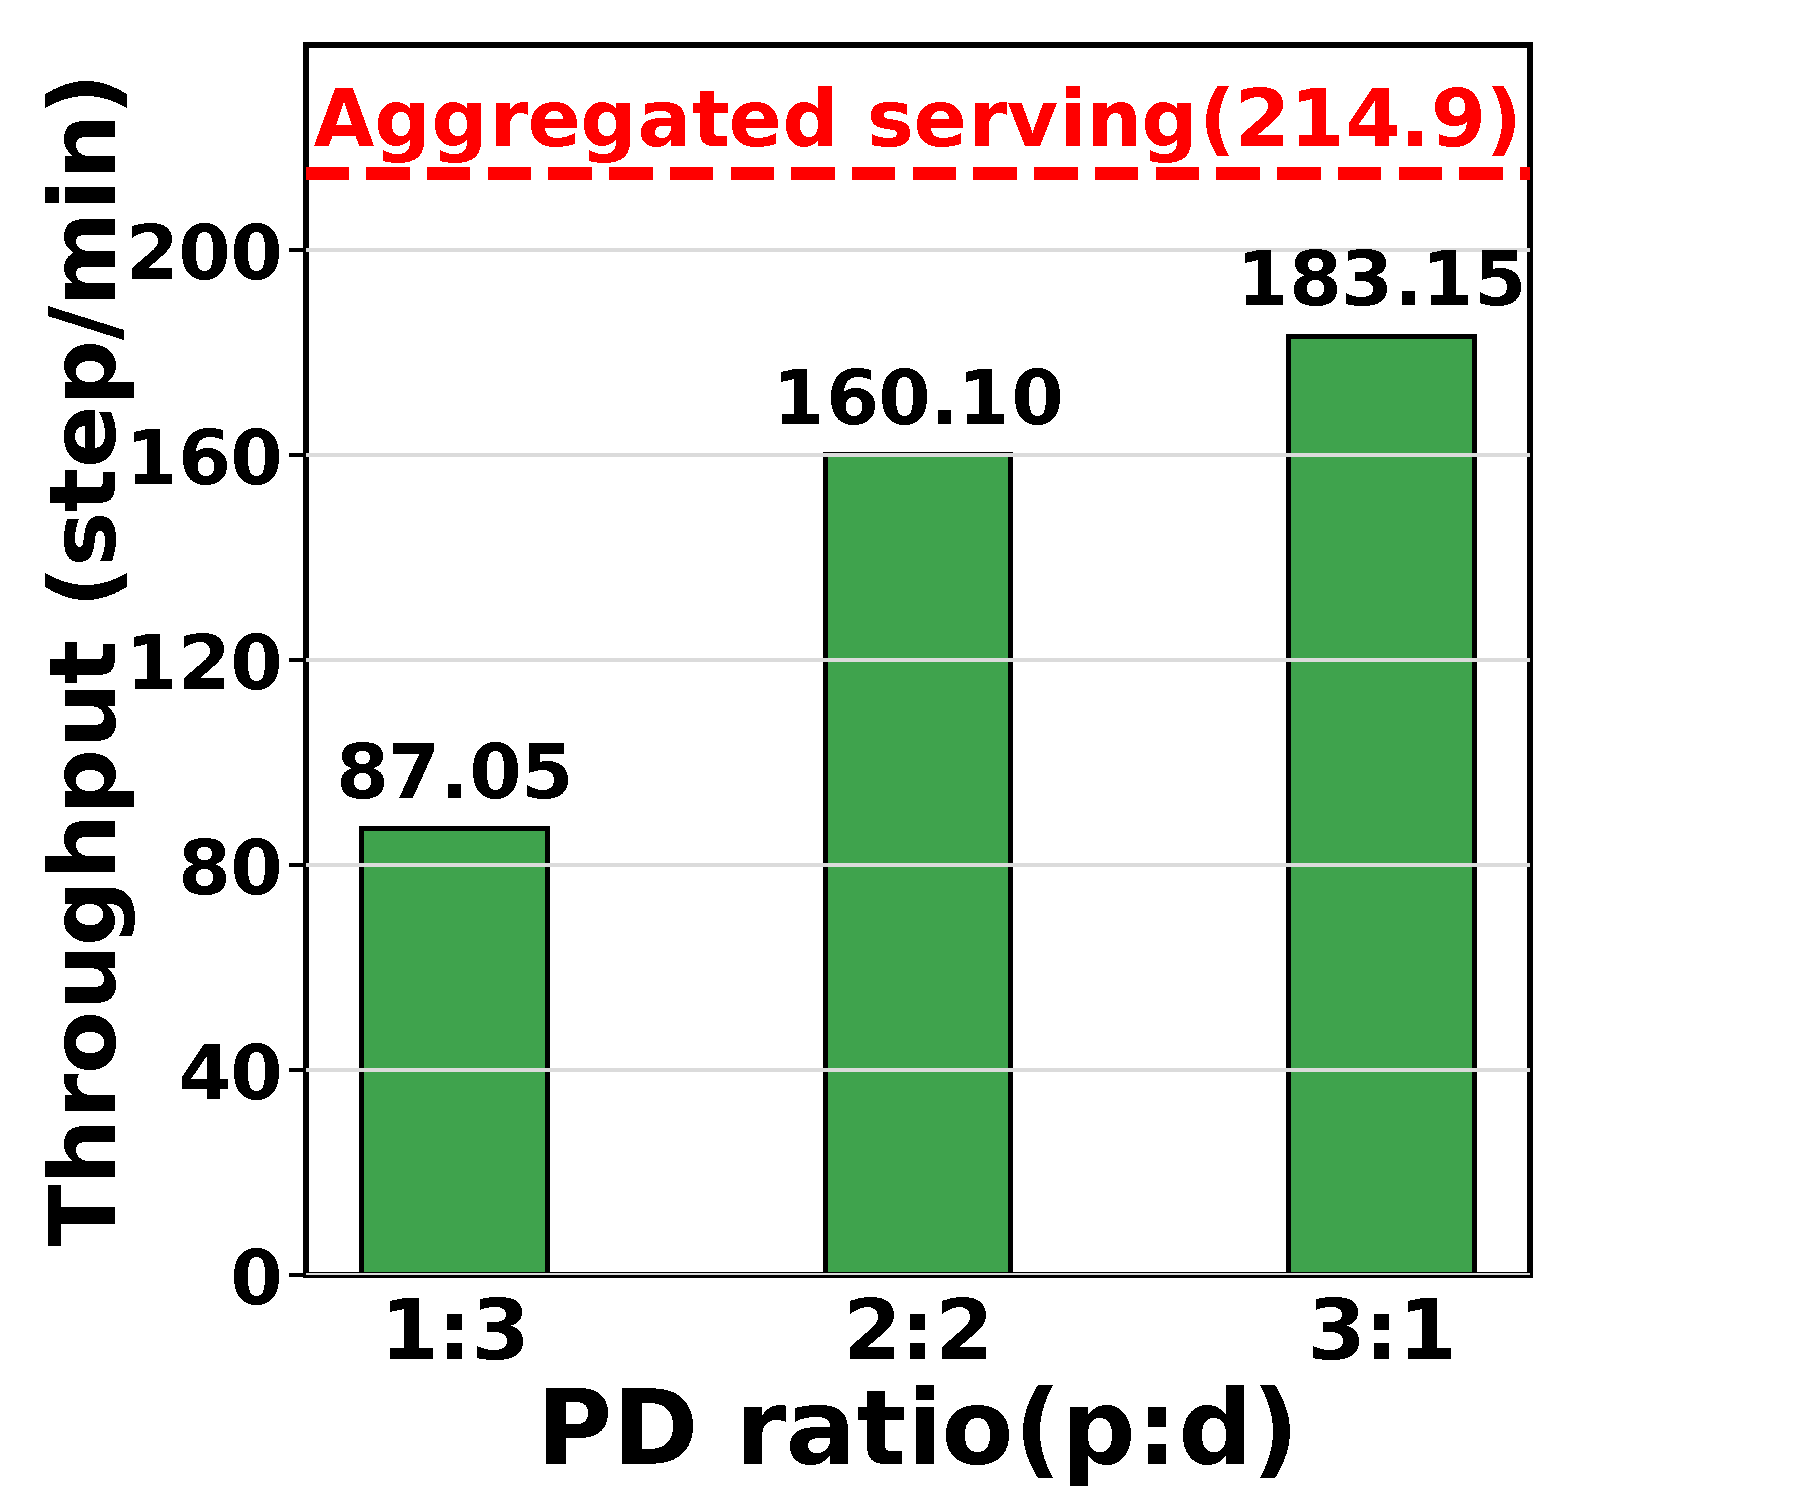
\includegraphics[width=0.99\linewidth]{Figures/throughput_vs_pd_ratio.pdf}
        \caption{吞吐量对比Prefill-Only/Decode-Only Node Ratio}
        \label{fig:throughput_pd}
    \end{subfigure}

    \caption{KV 缓存卸载和预填充解码（PD）分解的消融研究}
    \label{fig:both_figures}
\end{figure}



\subsection{扩大智能体工作流}
\label{sec:rl_scale}
\textbf{异构资源分配和调度。}
为了大规模协调多轮智能体与环境的交互，最近的系统（例如 MegaFlow~）\cite{zhang2026megaflow}, RollArt~\cite{gao2025rollart,wang2025let},AgentRL~\cite{zhang2025agentrl}、VerlTool~\cite{jiang2025verltool} 将模型推理与环境执行分离。虽然这些框架通过专门的服务有效地扩展了环境并发性，但它们表现出了粗粒度分解的固有局限性。这些系统将推理引擎和工具执行器视为孤立的黑匣子，缺乏统一的资源管理，无法协调KV 缓存生命周期与环境执行。如果没有程序级的细粒度调度，基于分解的方法会浪费智能体工作负载中的 KV 缓存重用潜力，从而产生次优吞吐量。

\newpage

\section{系统可移植性和接口抽象。}
\label{app:easy_intergrate}
\subsection{中间件架构和统一接口。}
\noindent \ouralg 充当 \textbf{程序感知运行时层} 通过程序级抽象在智能体控制流和后端推理引擎之间进行调解。调度器根据抽象的状态控制程序状态转换 \texttt{ProgramState} （见表~\ref{tab:program-state}）连同后端缓存容量视图（见表~\ref{tab:backend-state}）。同时，每个程序仅绑定到端点，不依赖于具体的后端实现。

\subsection{为什么程序 ID 很重要。}

虽然标准 \textbf{会话 ID} 作为路由标签， \textbf{我们的系统使用程序 ID 来检查工作流元数据。} 这种可见性至关重要：它允许调度器区分有效的工具等待时间和空闲会话，从而实现基于会话的基线无法支持的智能抢占策略。

\subsection{ThunderAgent 的低开销采用。}
图~\ref{fig:router-minimal-changes} 表明采用ThunderAgent \textbf{只需要} 附着 \texttt{program\_id} 请求（LLM 推理和工具执行）并发送明确的释放信号 \texttt{program\_id} 当一个程序结束时。
这 \texttt{program\_id} 用自己的程序实例标记每个请求以进行调度，而
释放信号允许 ThunderAgent 在终止后回收每个程序的资源。
\textbf{所有其他请求字段和 OpenAI 风格的 API 界面保持不变。}

%pipeline contradiction


%program state table
\begin{table}[!htbp]
\centering
\footnotesize
\setlength{\tabcolsep}{3pt}
\renewcommand{\arraystretch}{1.05}

\begin{subtable}[t]{0.56\linewidth}
\centering
\begin{tabular}{@{} l l p{0.54\linewidth} @{}}
\toprule
\textbf{场地} & \textbf{类型} & \textbf{意义} \\
\midrule
\multicolumn{3}{@{}l}{\textbf{程序状态}} \\
\addlinespace[2pt]
\texttt{status}        & 节目状态 & 当前生命周期状态。 \\
\texttt{backend\_url}  & 斯特           & 分配的后端端点。 \\
\texttt{step\_count}   & 整数           & 到目前为止已执行的步骤。 \\
\texttt{total\_tokens} & 整数           & 完整历史记录中的代币总数。 \\
\bottomrule
\end{tabular}
\subcaption{程序状态字段。}
\label{tab:program-state}
\end{subtable}
\hfill
\begin{subtable}[t]{0.42\linewidth}
\centering
% key change: fixed-width first column + explicit gap + remaining-width second column
\begin{tabular}{@{} >{\raggedright\arraybackslash}p{0.34\linewidth}
                @{\hspace{10pt}}
                >{\raggedright\arraybackslash}p{0.56\linewidth} @{}}
\toprule
\textbf{地位} & \textbf{意义} \\
\midrule
\multicolumn{2}{@{}l}{\textbf{节目状态}} \\
\addlinespace[2pt]
\texttt{REASONING} & GPU 上的推理。 \\
\texttt{ACTING}    & Off-GPU 工具执行程序。 \\
\texttt{PAUSED}    & 在全局暂停等待集中。 \\
\texttt{STOPPED}   & 已发布；资源被回收。 \\
\bottomrule
\end{tabular}
\subcaption{程序状态语义。}
\label{tab:program-status}
\end{subtable}

\caption{程序状态和状态定义。}
\label{tab:program-state-status}
\end{table}

%backend state table
\begin{table}[!htbp]
\centering
\footnotesize
\setlength{\tabcolsep}{3pt}
\renewcommand{\arraystretch}{1.05}

\begin{tabular}{@{} l l p{6.2cm} @{}}
\toprule
\textbf{场地} & \textbf{类型} & \textbf{意义} \\
\midrule
\multicolumn{3}{@{}l}{\textbf{后端状态}} \\
\addlinespace[2pt]
\texttt{url} & 斯特 & 后端端点。 \\
\texttt{healthy} & 布尔值 & 用于调度的健康标志。 \\
\texttt{cache\_config} & 可选[缓存配置] & 静态缓存配置（在启动时获取）。 \\
\texttt{active\_program\_tokens} & 整数 & 此后端上的活动令牌足迹。 \\
\bottomrule
\end{tabular}

\vspace{6pt} % <-- increase to push caption further down
\caption{BackendState 的关键字段。}
\label{tab:backend-state}

\end{table}

\begin{figure}[!htbp]
\centering

\begin{minipage}[t]{0.485\linewidth}
\centering
\textbf{仅推理后端（例如 vLLM/SGLang）}\\[-2pt]
\begin{tcolorbox}[
  colback=black!3,
  colframe=black!35,
  boxrule=0.4pt,
  arc=1.2pt,
  left=4pt,right=4pt,top=3pt,bottom=3pt
]
\begin{lstlisting}[style=req]
(*@\textcolor{blue!70!black}{\# 1) LLM request}@*)
chat_completion(model_id, messages, extrabody)

(*@\textcolor{blue!70!black}{\# 2) Tool execution}@*)
run_tool(command, sandbox)

(*@\textcolor{blue!70!black}{\# 3) Program end}@*)
# (no explicit release)
\end{lstlisting}
\end{tcolorbox}
\end{minipage}
\hfill
\begin{minipage}[t]{0.485\linewidth}
\centering
\textbf{With ThunderAgent}\\[-2pt]
\begin{tcolorbox}[
  colback=black!3,
  colframe=black!35,
  boxrule=0.4pt,
  arc=1.2pt,
  left=4pt,right=4pt,top=3pt,bottom=3pt
]
\begin{lstlisting}[style=req]
(*@\textcolor{orange!80!black}{\# 1) LLM request}@*)
extrabody[(*@\textbf{"program\_id"}@*)] = "PID"
chat_completion(model_id, messages, extrabody)

(*@\textcolor{orange!80!black}{\# 2) Tool execution}@*)
run_tool(command, sandbox, (*@\textbf{program\_id="PID"}@*))

(*@\textcolor{orange!80!black}{\# 3) Program end (explicit release)}@*)
POST /programs/release
{ (*@\textbf{"program\_id"}@*): "PID" }
\end{lstlisting}
\end{tcolorbox}
\end{minipage}

\caption{\textbf{使用 ThunderAgent 只需要进行三处更改。}}
\label{fig:router-minimal-changes}
\end{figure}






\newpage
\section{工具执行时间可变性。}
\label{app:tool_var}

\noindent\textbf{实际的智能体工具调用很难表征并且通常是不可预测的。} 在一些以代码为中心的设置中（例如，服务 SWE-Bench~\citep{jimenez2024swebenchlanguagemodelsresolve} 与SWE-Agent~\citep{yang2024sweagentagentcomputerinterfacesenable} 或OpenHands~\citep{wang2025openhandsopenplatformai}），智能体主要调用本地的轻量级工具，工具延迟相对稳定，方差较小。然而，在更广泛和更现实的场景中，例如服务 HLE~\citep{phan2025humanitysexam} 与 ToolOrchestra 一起~\citep{su2025toolorchestraelevatingintelligenceefficient}，工作负载更加依赖远程服务工具（表~\ref{tab:tool-buckets}），使得工具执行时间不稳定且难以预测。这种波动很大程度上源于智能体运行时的外部因素，例如网络抖动、后端负载和排队延迟以及速率限制，这些因素可能会因请求和时间而变化。

我们凭经验证实了图中的这种行为~\ref{fig:tool_time}。对于远程服务工具（以及一些执行工具），中位数和尾分位数之间的差距很大：p95和p99大大高于中位数，并且尾部可以延长到数十甚至数百秒。这表明这些设置中的工具延迟缺乏稳定的集中趋势；相反，重尾行为占主导地位， \textbf{使得工具延迟预测在实践中本质上很脆弱。}

考虑到工具执行的不可预测性，低估会浪费固定的缓存容量，同时仍然会触发过早的 KV 驱逐，导致恢复时出现抖动。相反，高估可能会导致不必要地驱逐本应保留的程序的 KV。即使工具运行时间是完全可预测的，现有的方法（例如Continuum）~\cite{li2025continuumefficientrobustmultiturn} 仍然决定是否使用静态的、基于阈值的规则来保持 KV 缓存固定。相比之下，ThunderAgent 构建 \textbf{完整的成本建模框架} 和 \textbf{动态权衡} $\text{Cost}_{\text{recompute}}$ 和 $\text{Cost}_{\text{caching}}$.








\begin{table}[!htbp]
\centering
\small
\setlength{\tabcolsep}{8pt}
\begin{tabular}{l l l}
\toprule
\textbf{工具桶} & \textbf{角色} & \textbf{主要变异源} \\
\midrule
\texttt{HLE-search} & 检索证据 & 远程服务（网络延迟/速率限制） \\
\texttt{HLE-enhance-reasoning} & 模型即工具调用 & 远程服务 \\
\texttt{HLE-answer} & 最终一代 & 本地LLM推理 \\
\midrule
\texttt{SAB-execute\_bash} & 外壳执行 & 沙箱和 I/O \\
\texttt{SAB-execute\_ipython\_cell} & Python 单元格执行 & 程序运行时间 \\
\texttt{SAB-str\_replace\_editor} & 文件编辑 & 本地文件系统 \\
\texttt{SAB-task\_tracker} & 任务状态跟踪 & 本地文件系统 \\
\bottomrule
\end{tabular}
\vspace{6pt}
\caption{工具桶。}
\label{tab:tool-buckets}
\end{table}





\begin{figure*}[]
  \centering

  % ===================== Row 1: HLE (3/3 filled) =====================
  \begin{subfigure}[t]{0.32\textwidth}
    \centering
    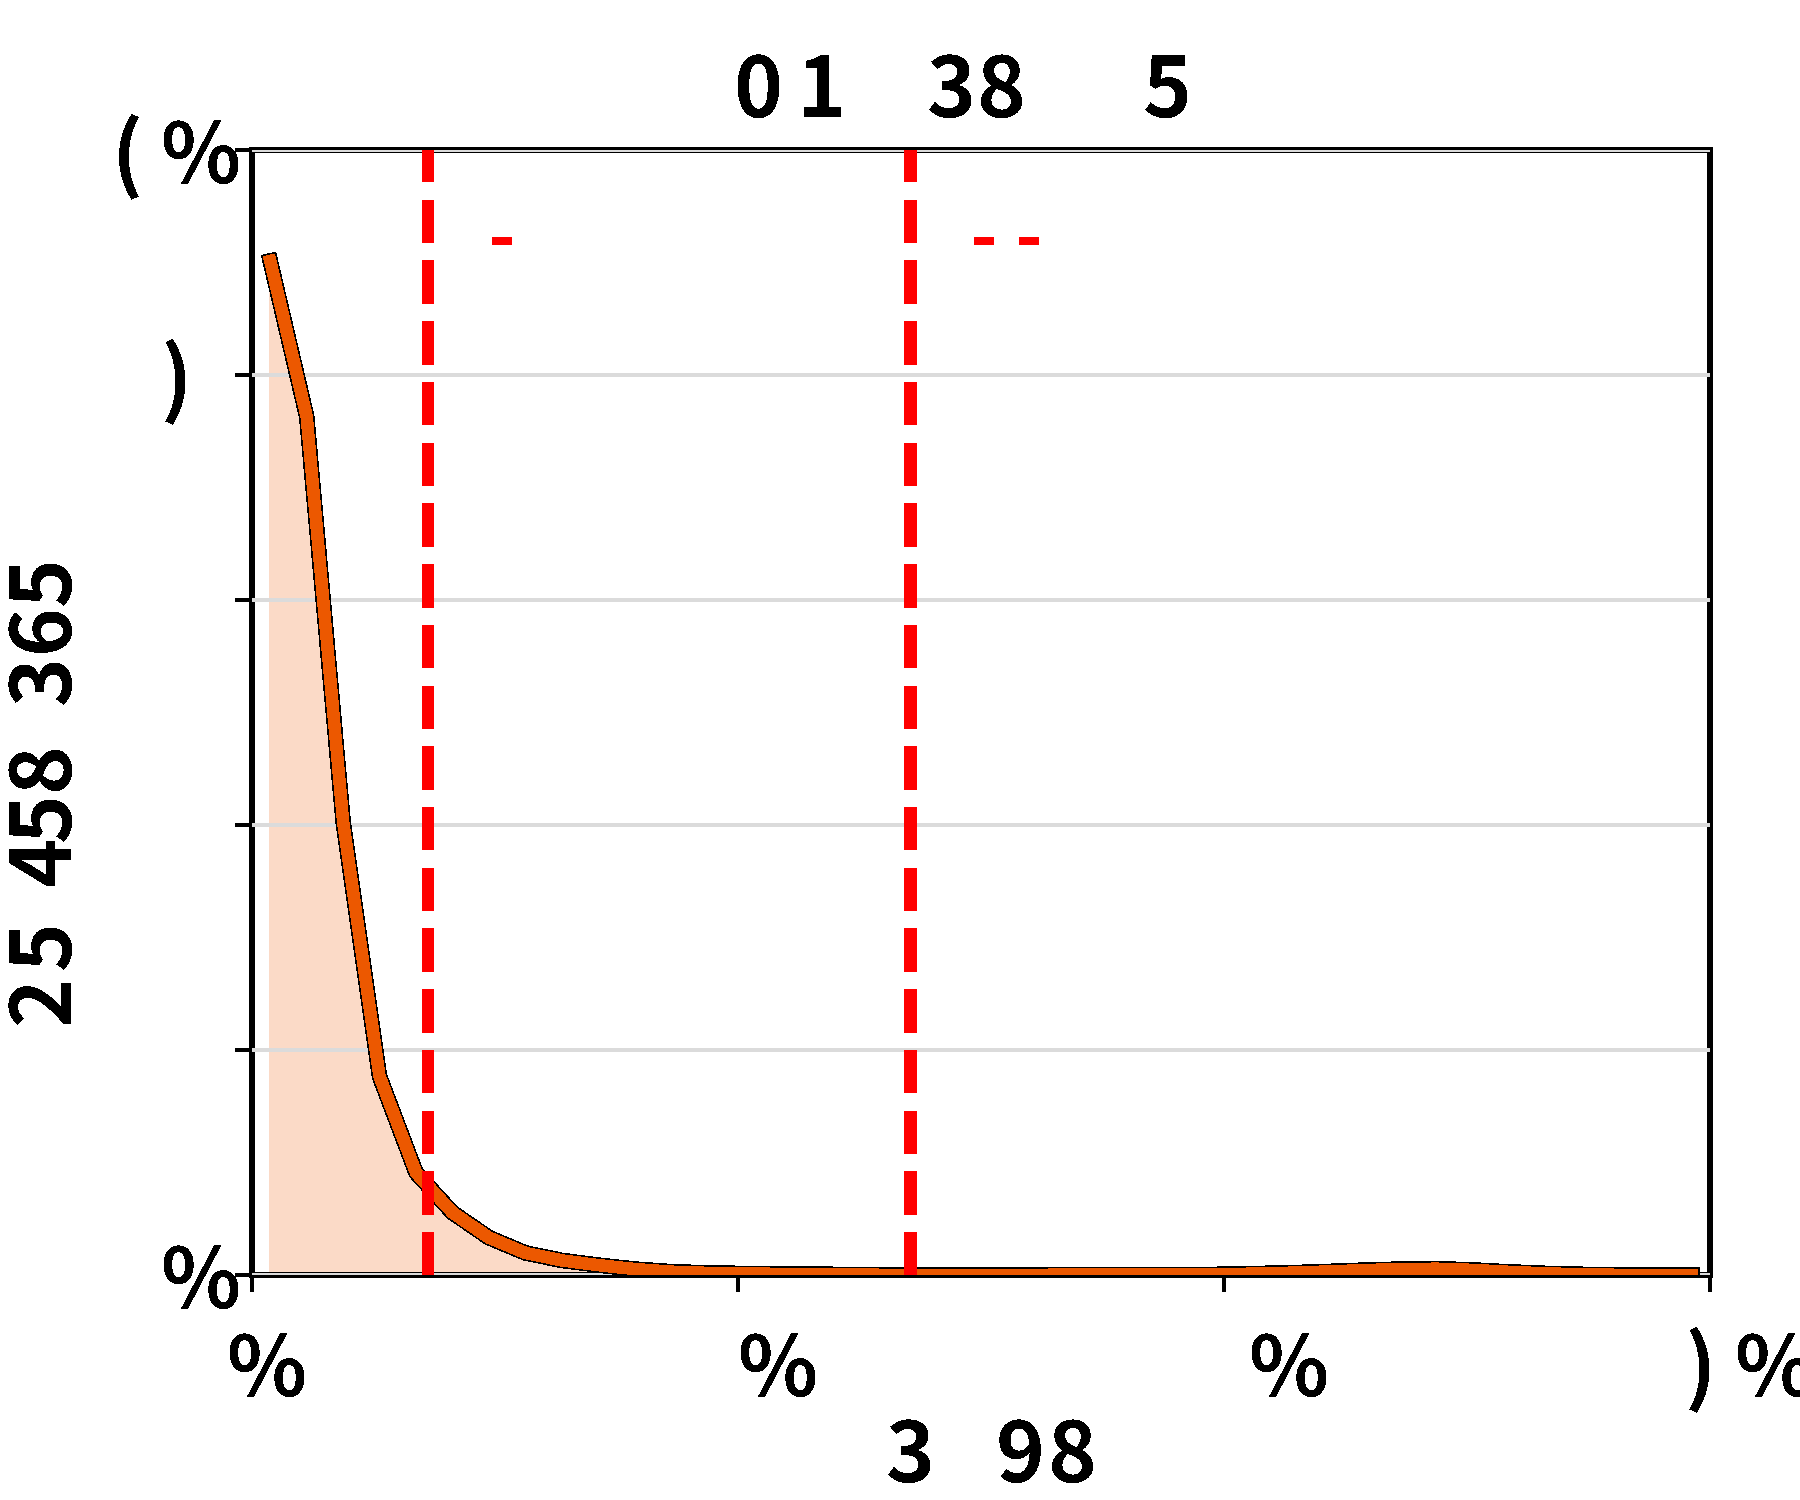
\includegraphics[width=0.8\linewidth ]{Figures/appendix_figs/hle_answer_latency_dist.pdf} % (a) optional
    \label{fig:hle_answer_latency}
  \end{subfigure}\hfill
  \begin{subfigure}[t]{0.32\textwidth}
    \centering
    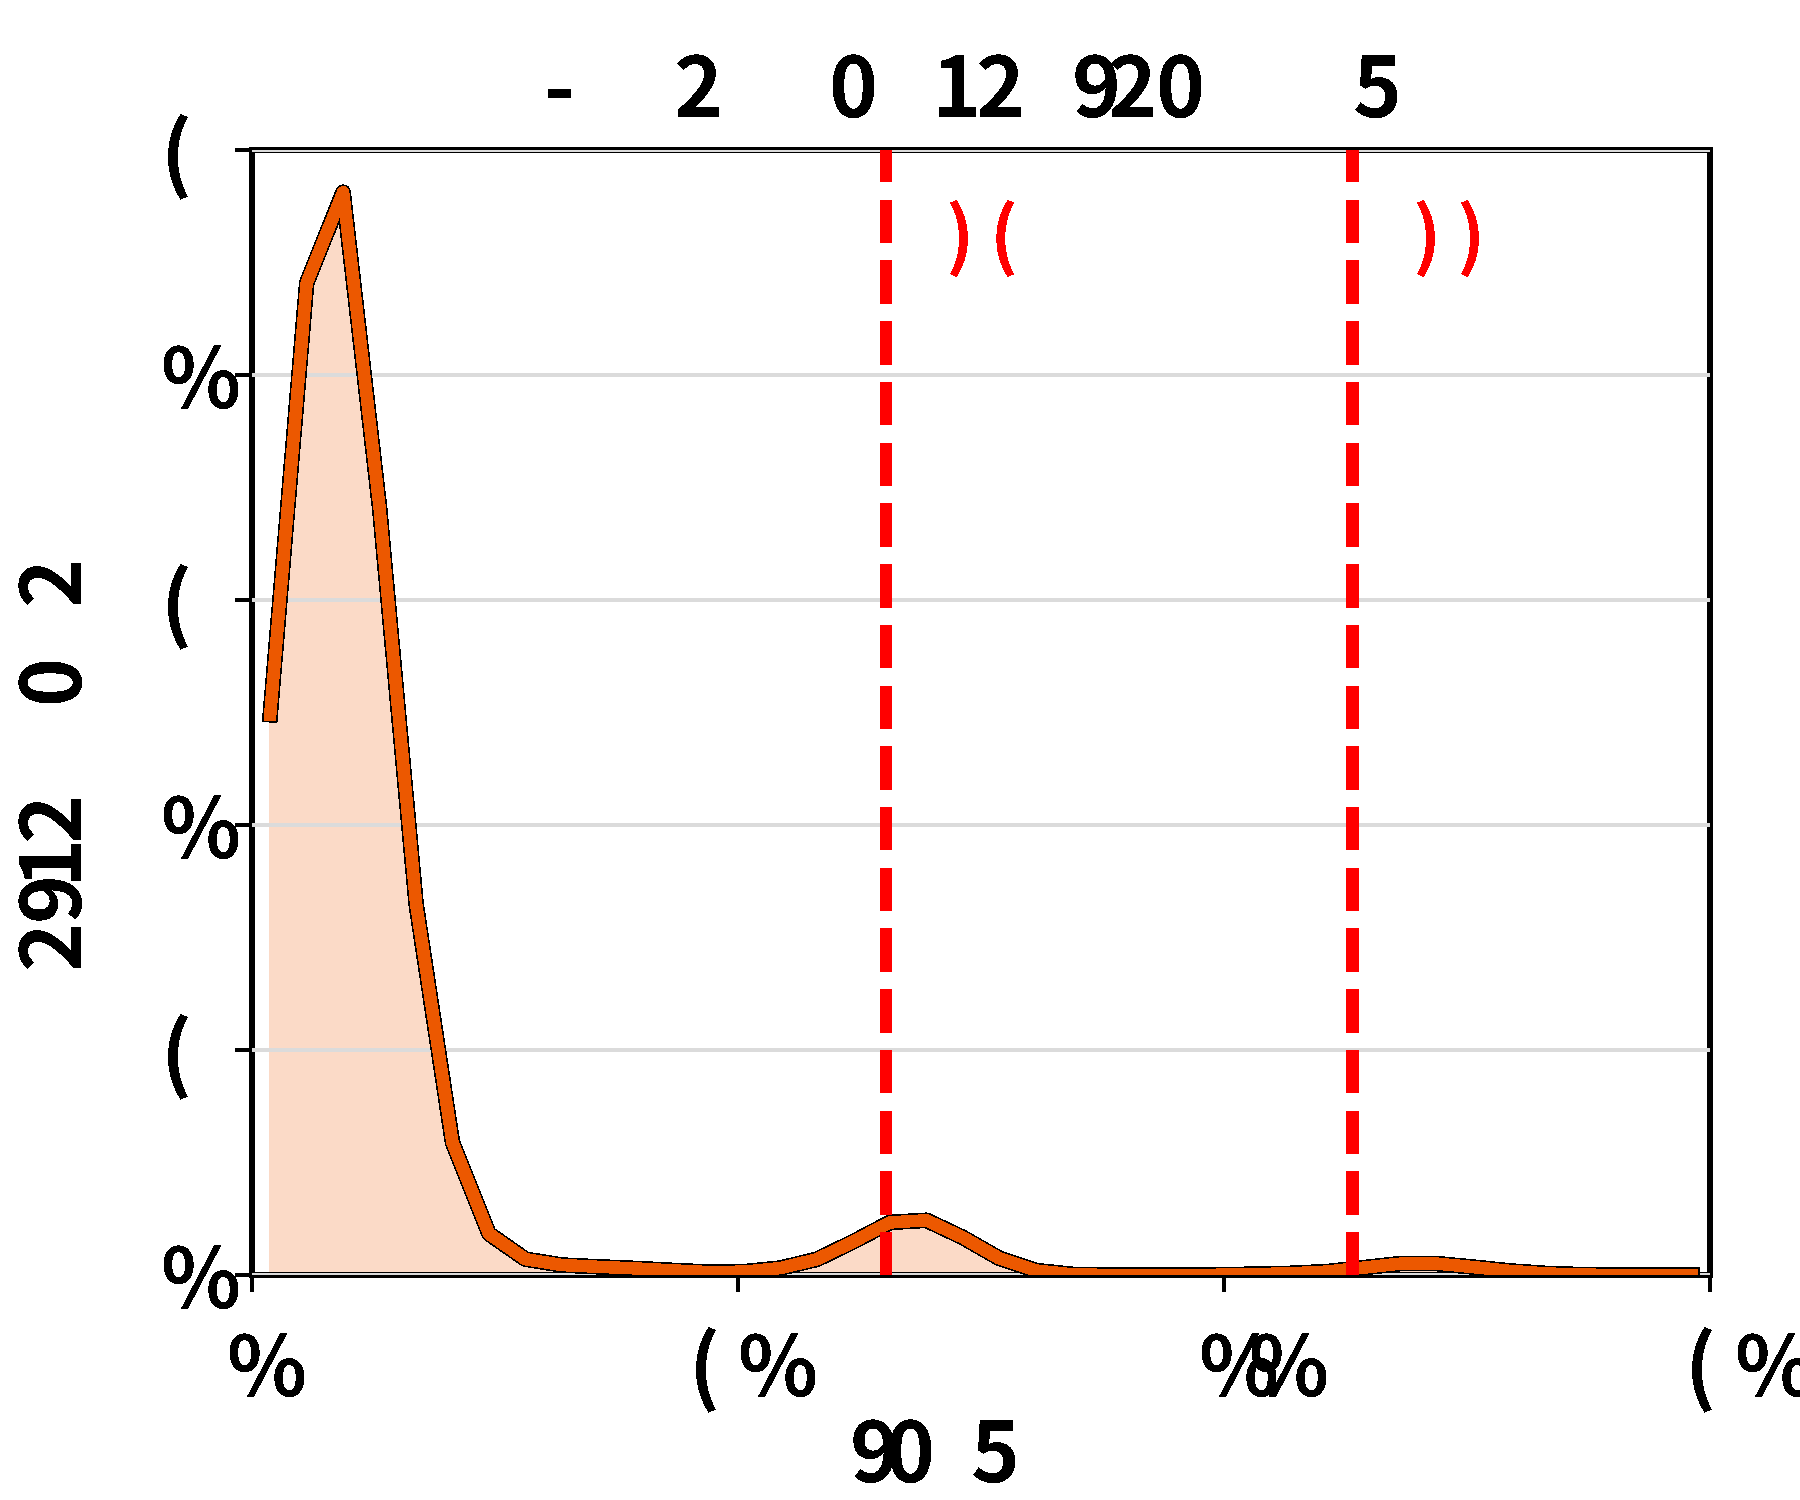
\includegraphics[width=0.8\linewidth ]{Figures/appendix_figs/hle_enhance_reasoning_latency_dist.pdf} % (b) optional
    \label{fig:hle_enhance_reasoning_latency}
  \end{subfigure}\hfill
  \begin{subfigure}[t]{0.32\textwidth}
    \centering
    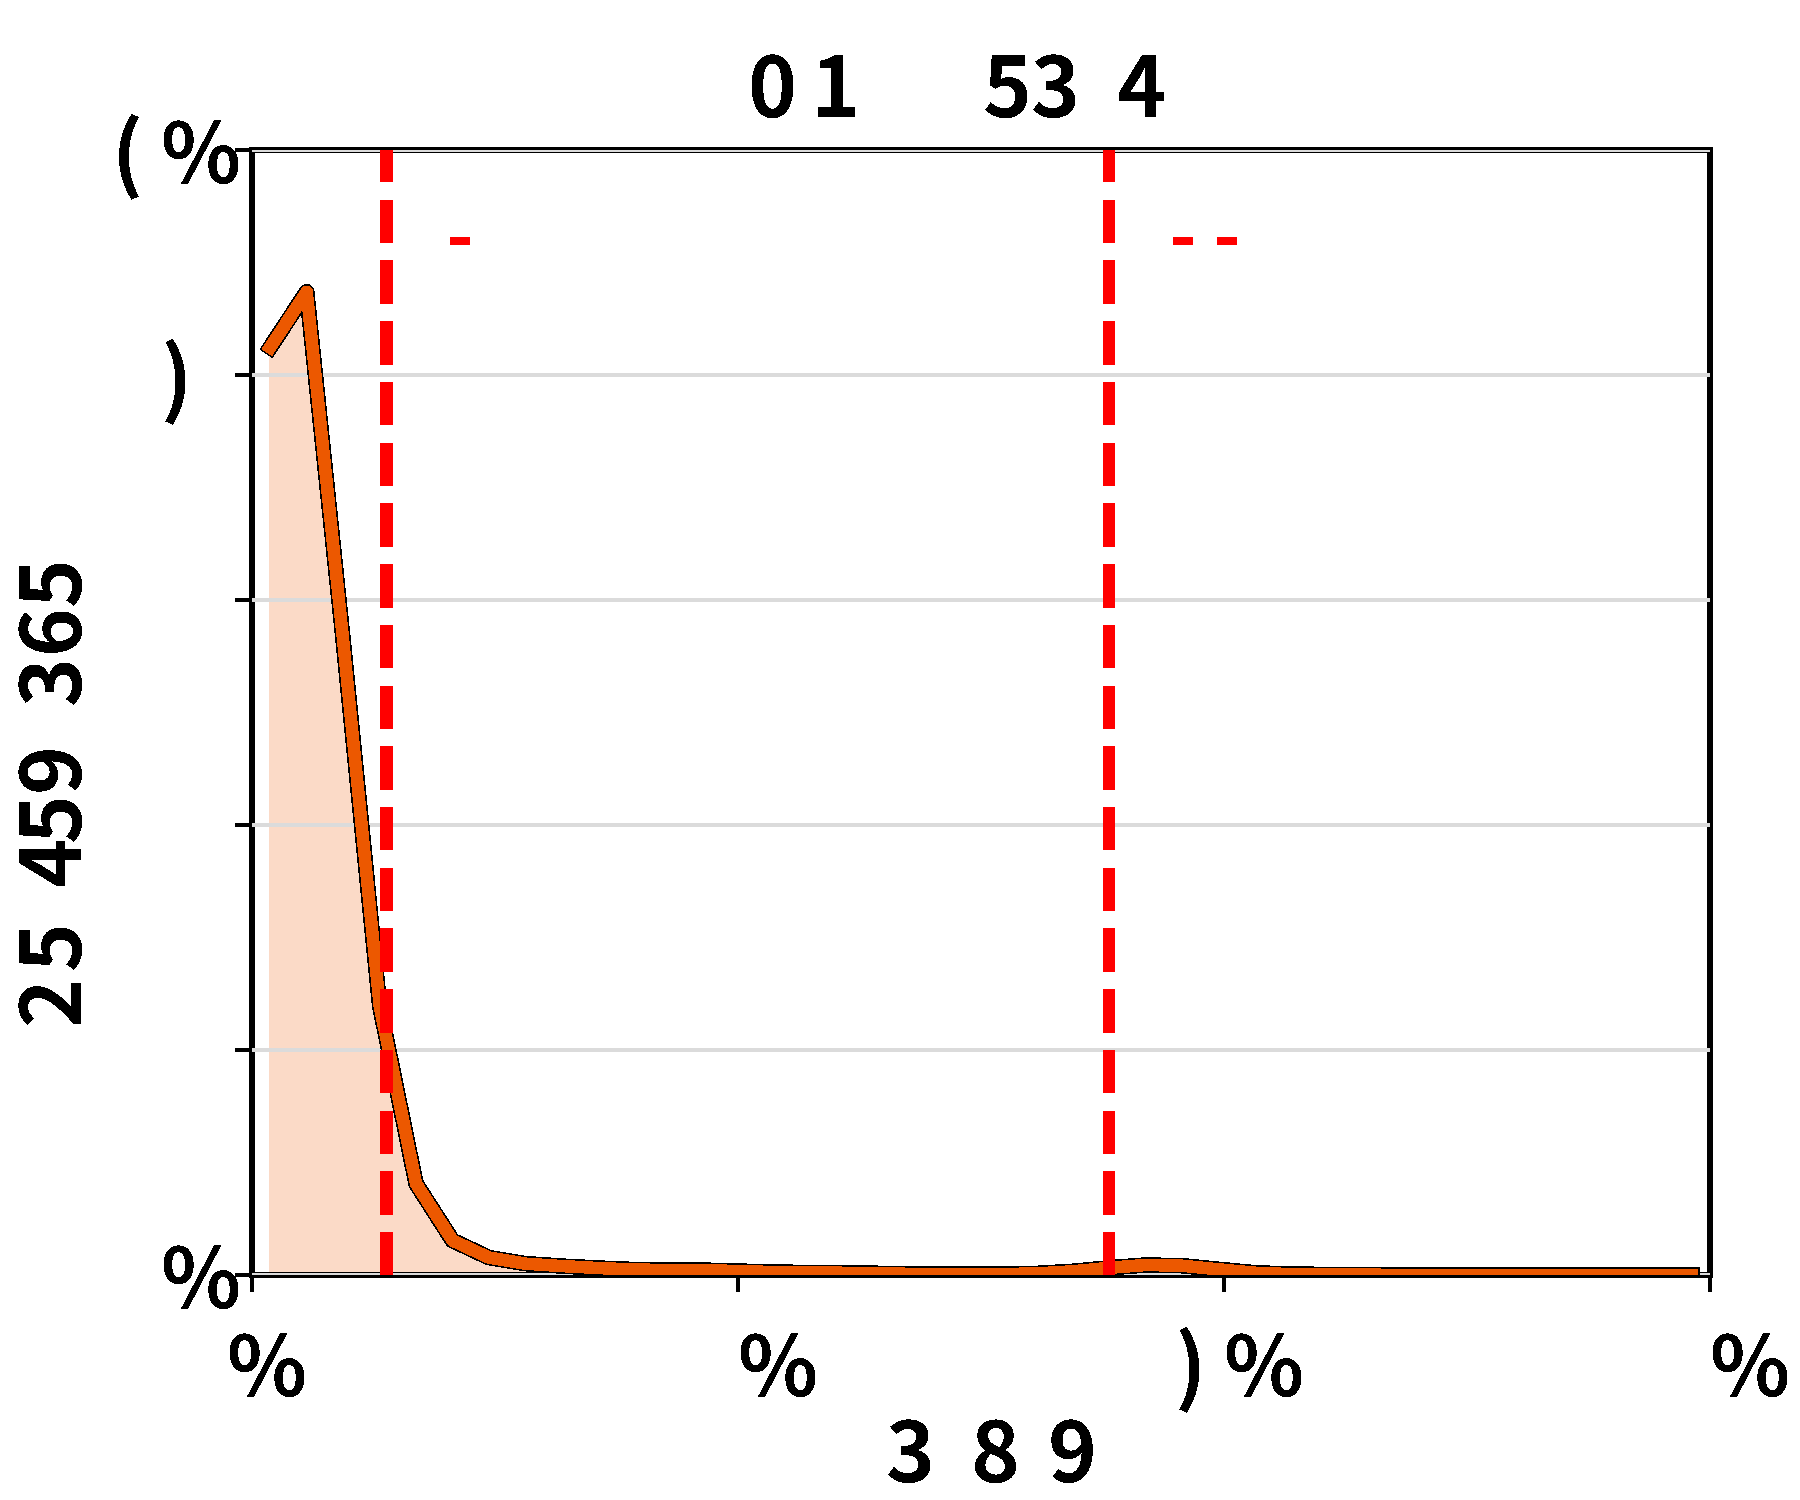
\includegraphics[width=0.8\linewidth ]{Figures/appendix_figs/hle_search_latency_dist.pdf} % (c) optional
    \label{fig:hle_search_latency}
  \end{subfigure}

  \vspace{2mm}

  % ===================== Row 2: SAB (now 3/3 filled) =====================
  \begin{subfigure}[t]{0.32\textwidth}
    \centering
    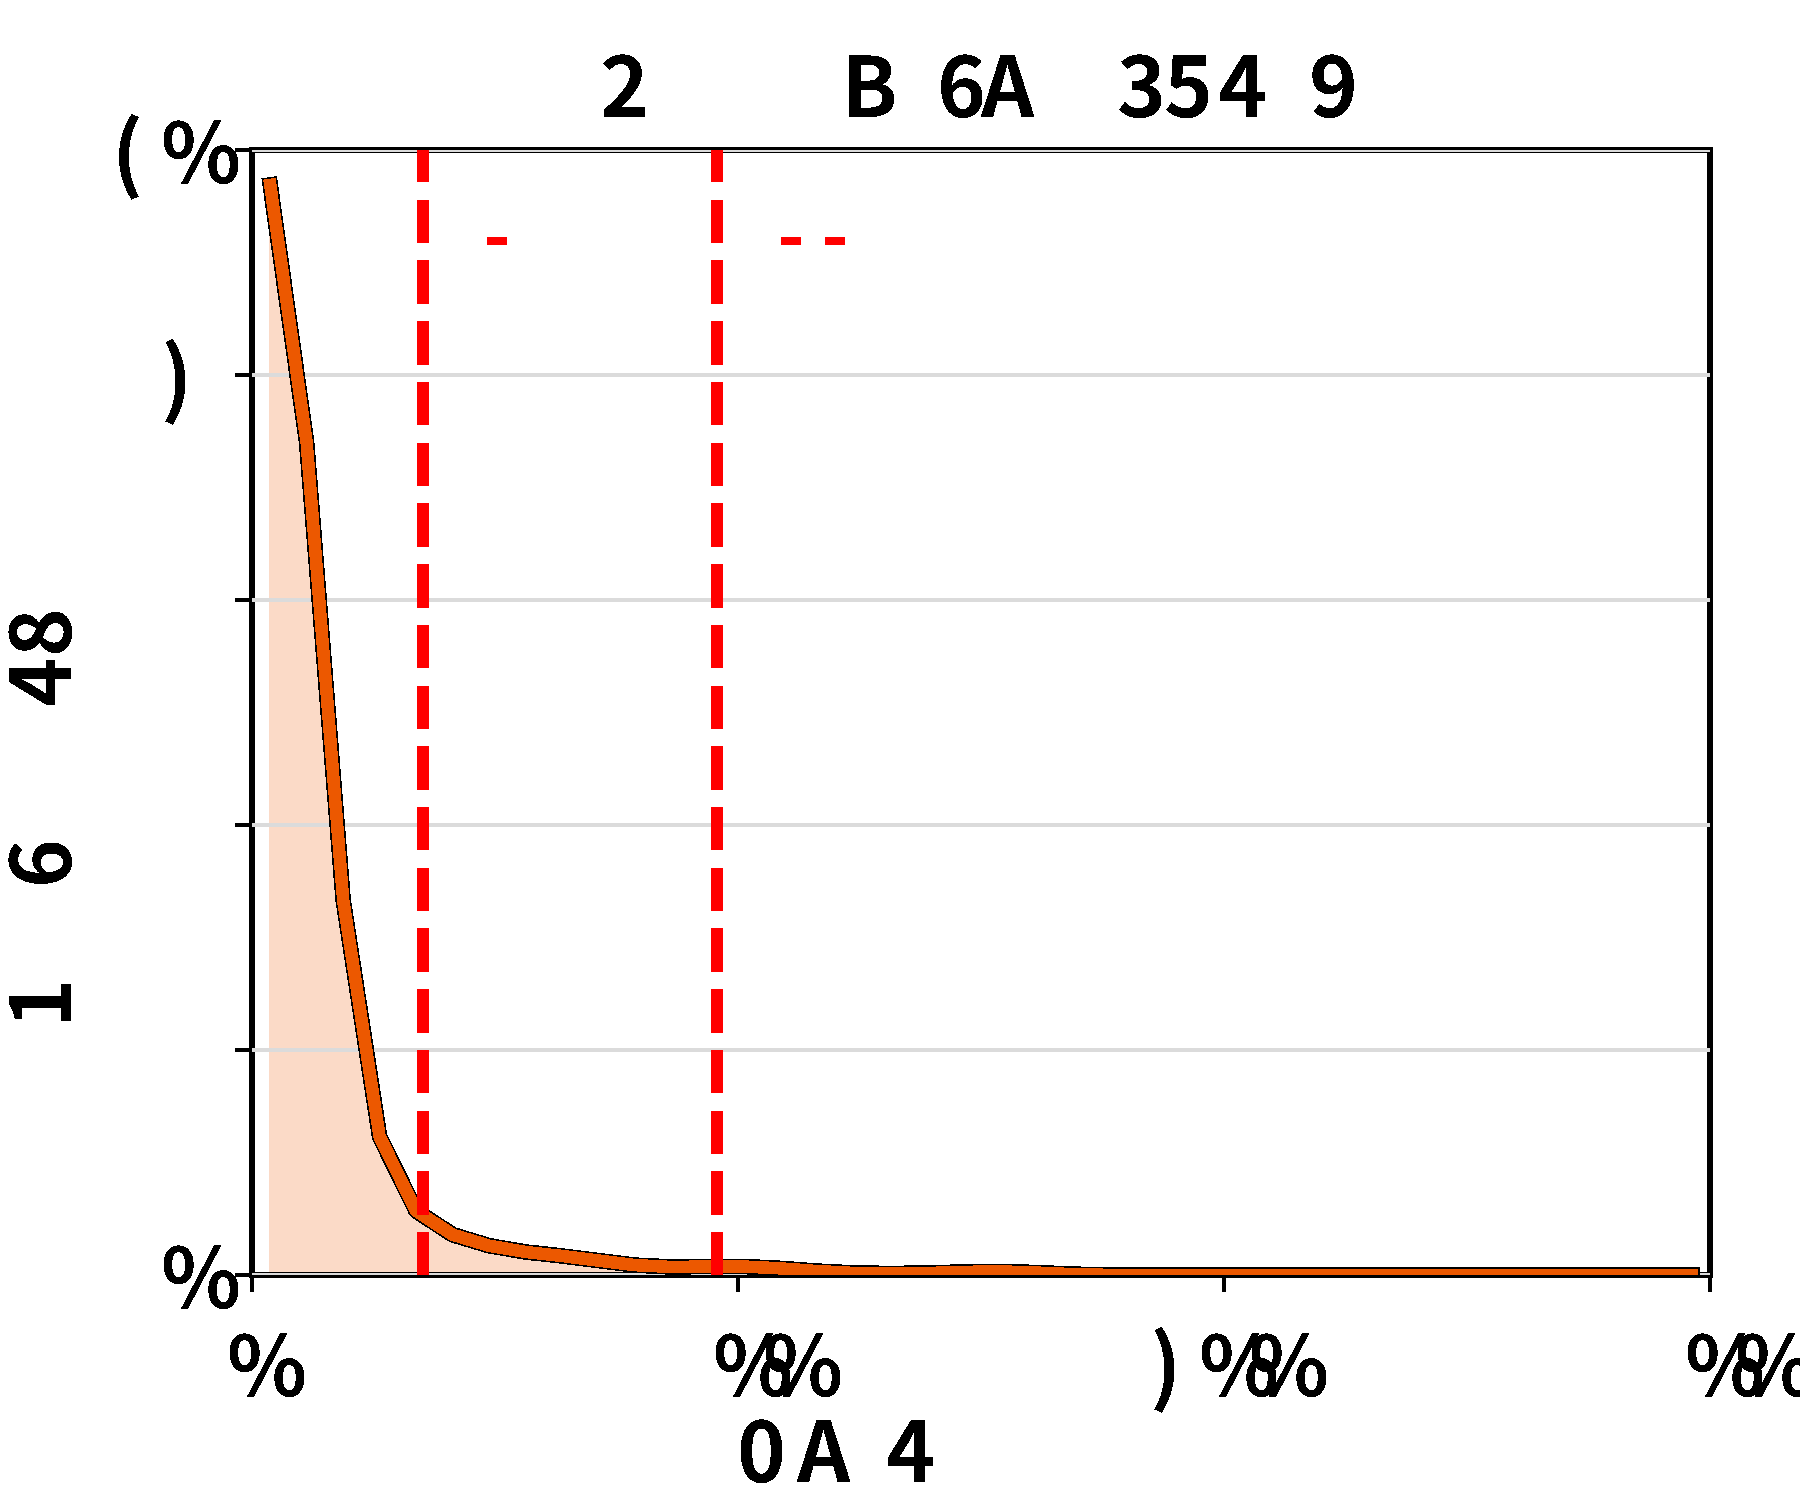
\includegraphics[width=0.8\linewidth ]{Figures/appendix_figs/sab_execute_bash_duration_dist.pdf} % (d) optional
    \label{fig:sab_execute_bash}
  \end{subfigure}\hfill
  \begin{subfigure}[t]{0.32\textwidth}
    \centering
    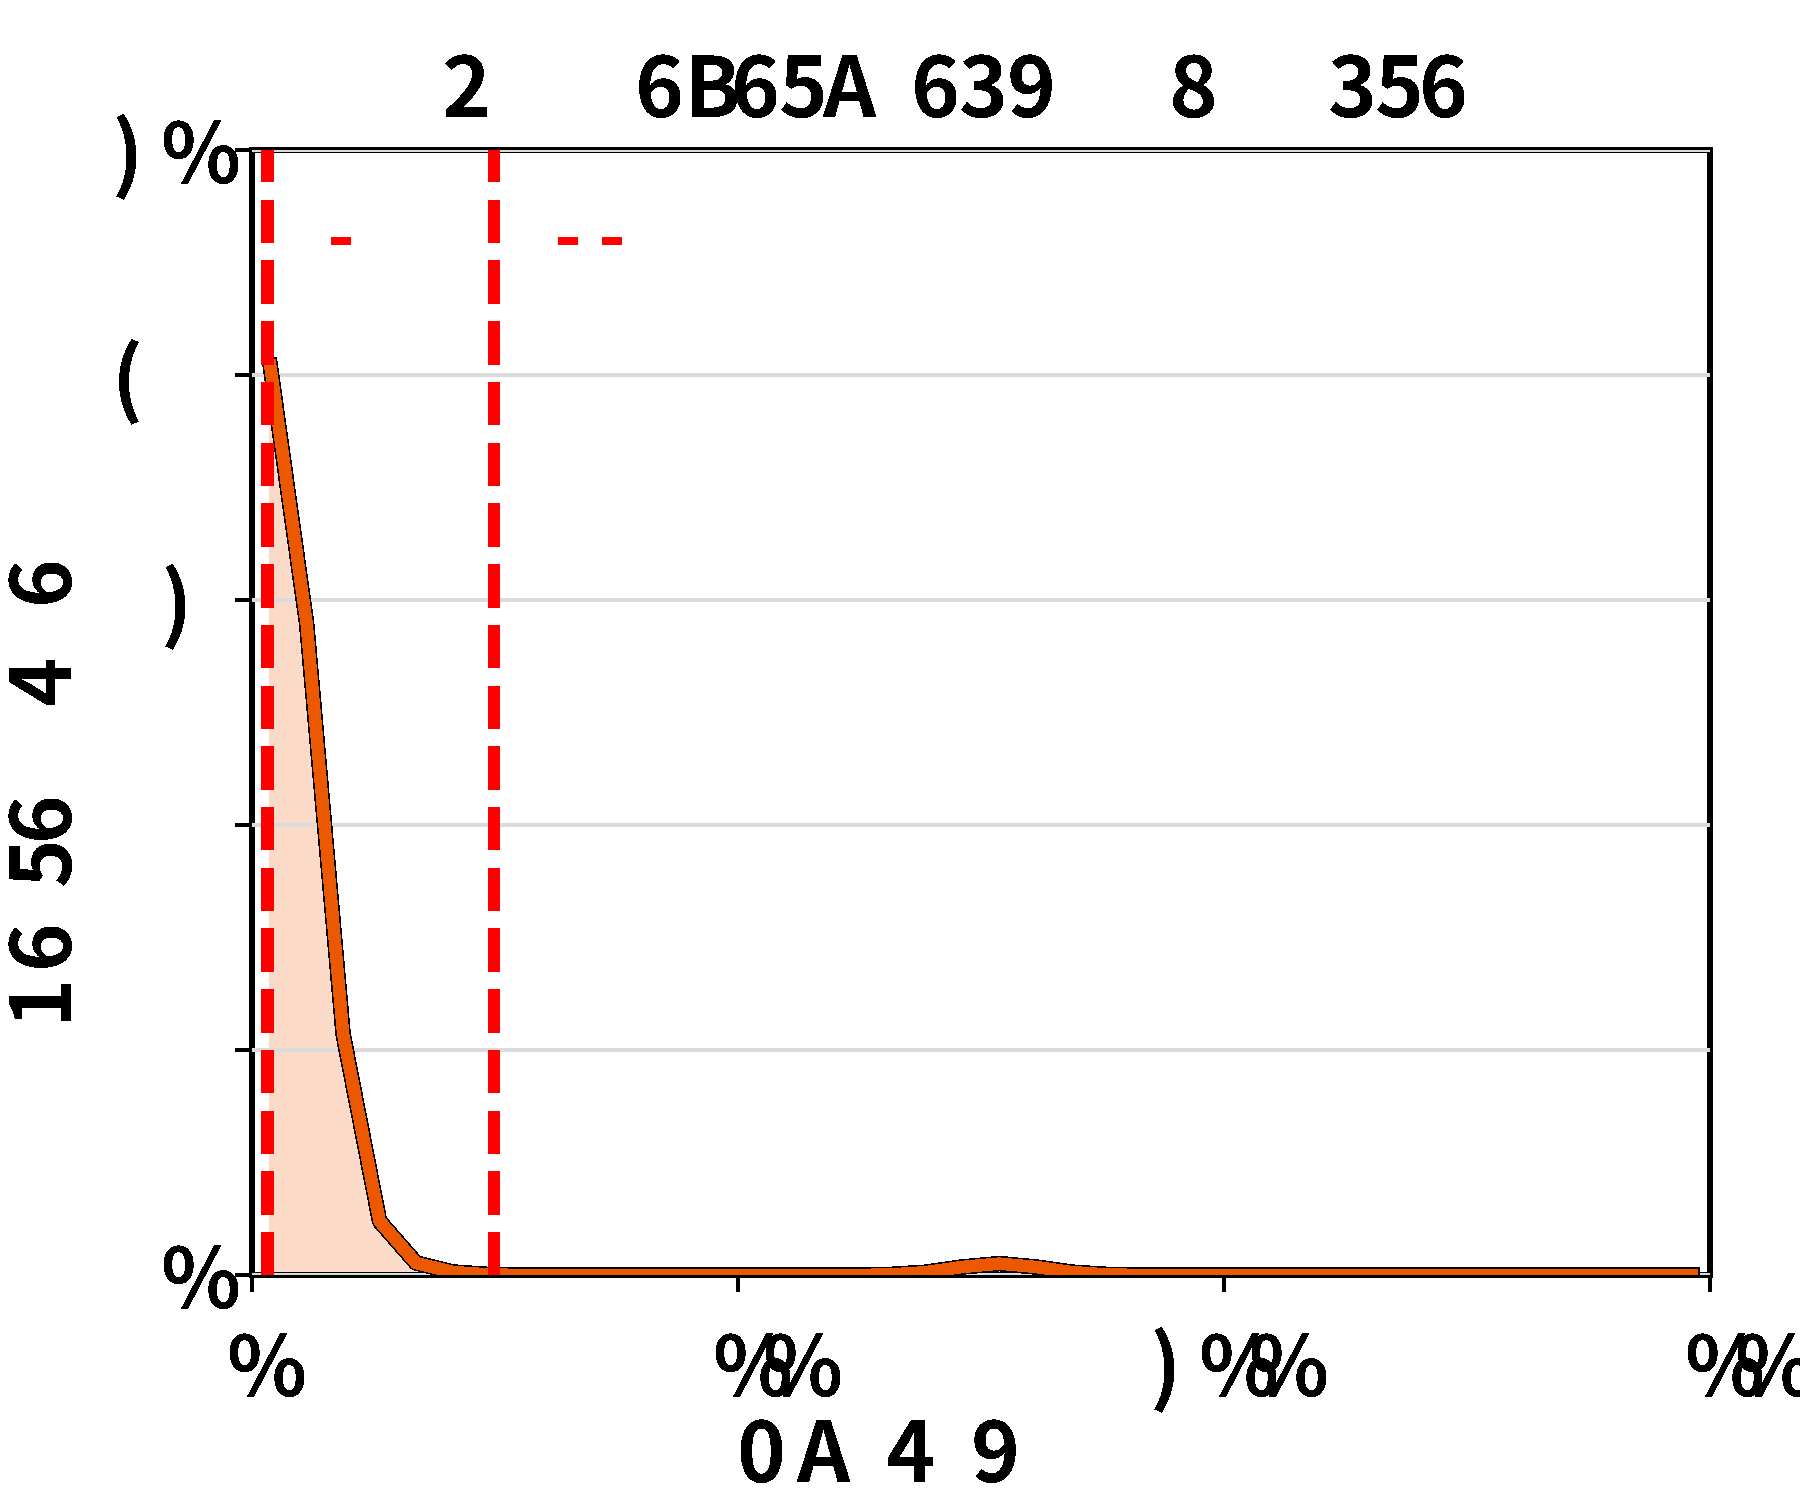
\includegraphics[width=0.8\linewidth ]{Figures/appendix_figs/sab_execute_ipython_cell_duration_dist.pdf} % (e) optional
    \label{fig:sab_execute_ipython}
  \end{subfigure}\hfill
  \begin{subfigure}[t]{0.32\textwidth}
    \centering
    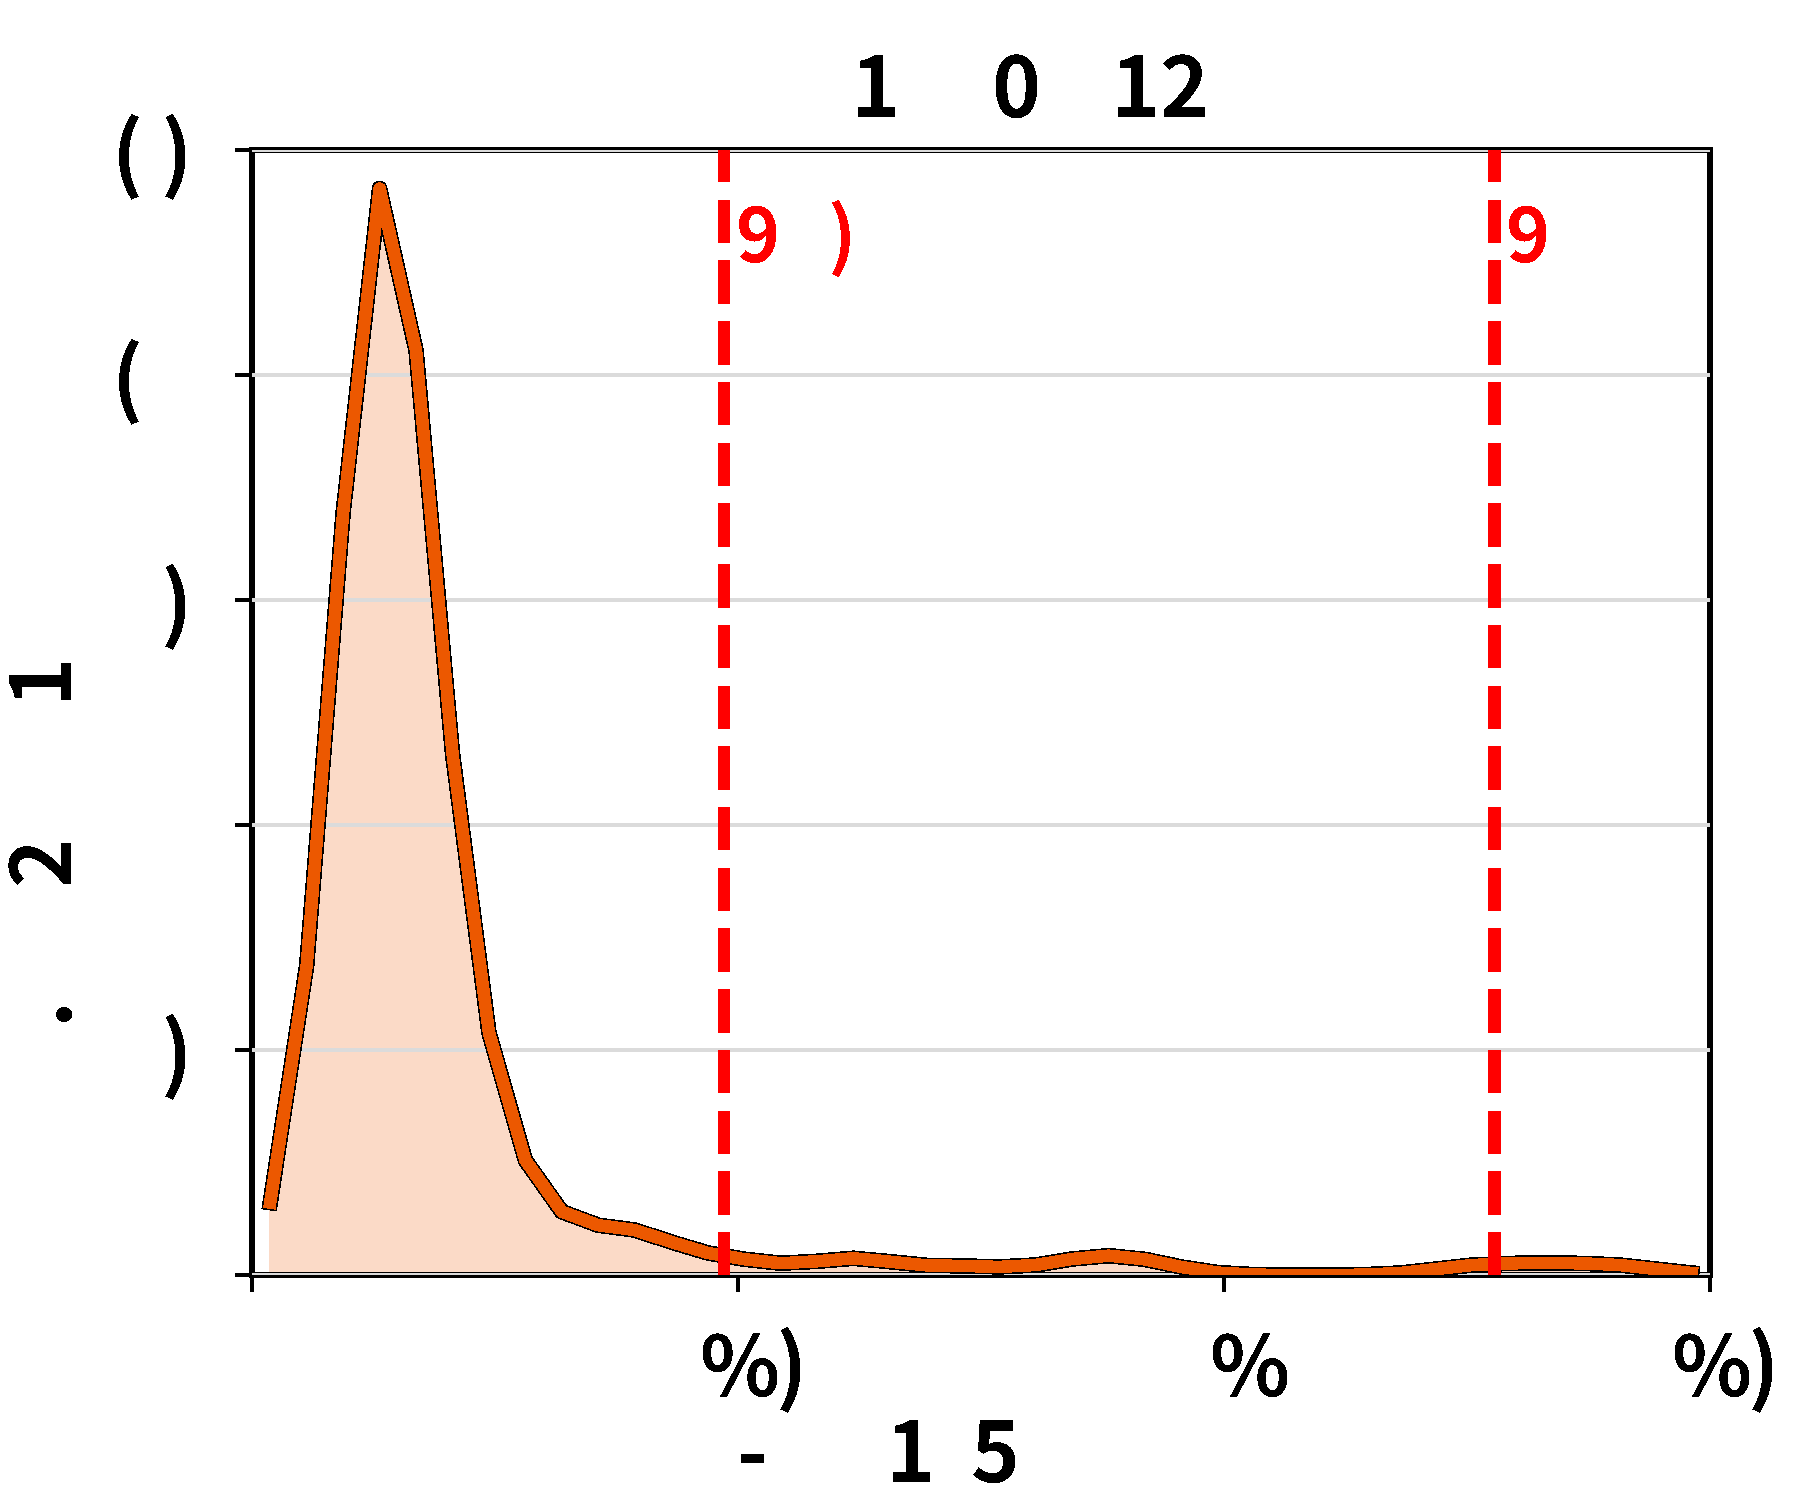
\includegraphics[width=0.8\linewidth ]{Figures/appendix_figs/sab_task_tracker_duration_dist.pdf}
    \label{fig:sab_task_tracker}
  \end{subfigure}

  \vspace{2mm}

  % ===================== Row 3: SAB (centered) =====================
  \begin{subfigure}[t]{0.32\textwidth}
    \centering
    % empty slot (keep layout)
    \label{fig:empty_slot_left}
  \end{subfigure}\hfill
  \begin{subfigure}[t]{0.32\textwidth}
    \centering
    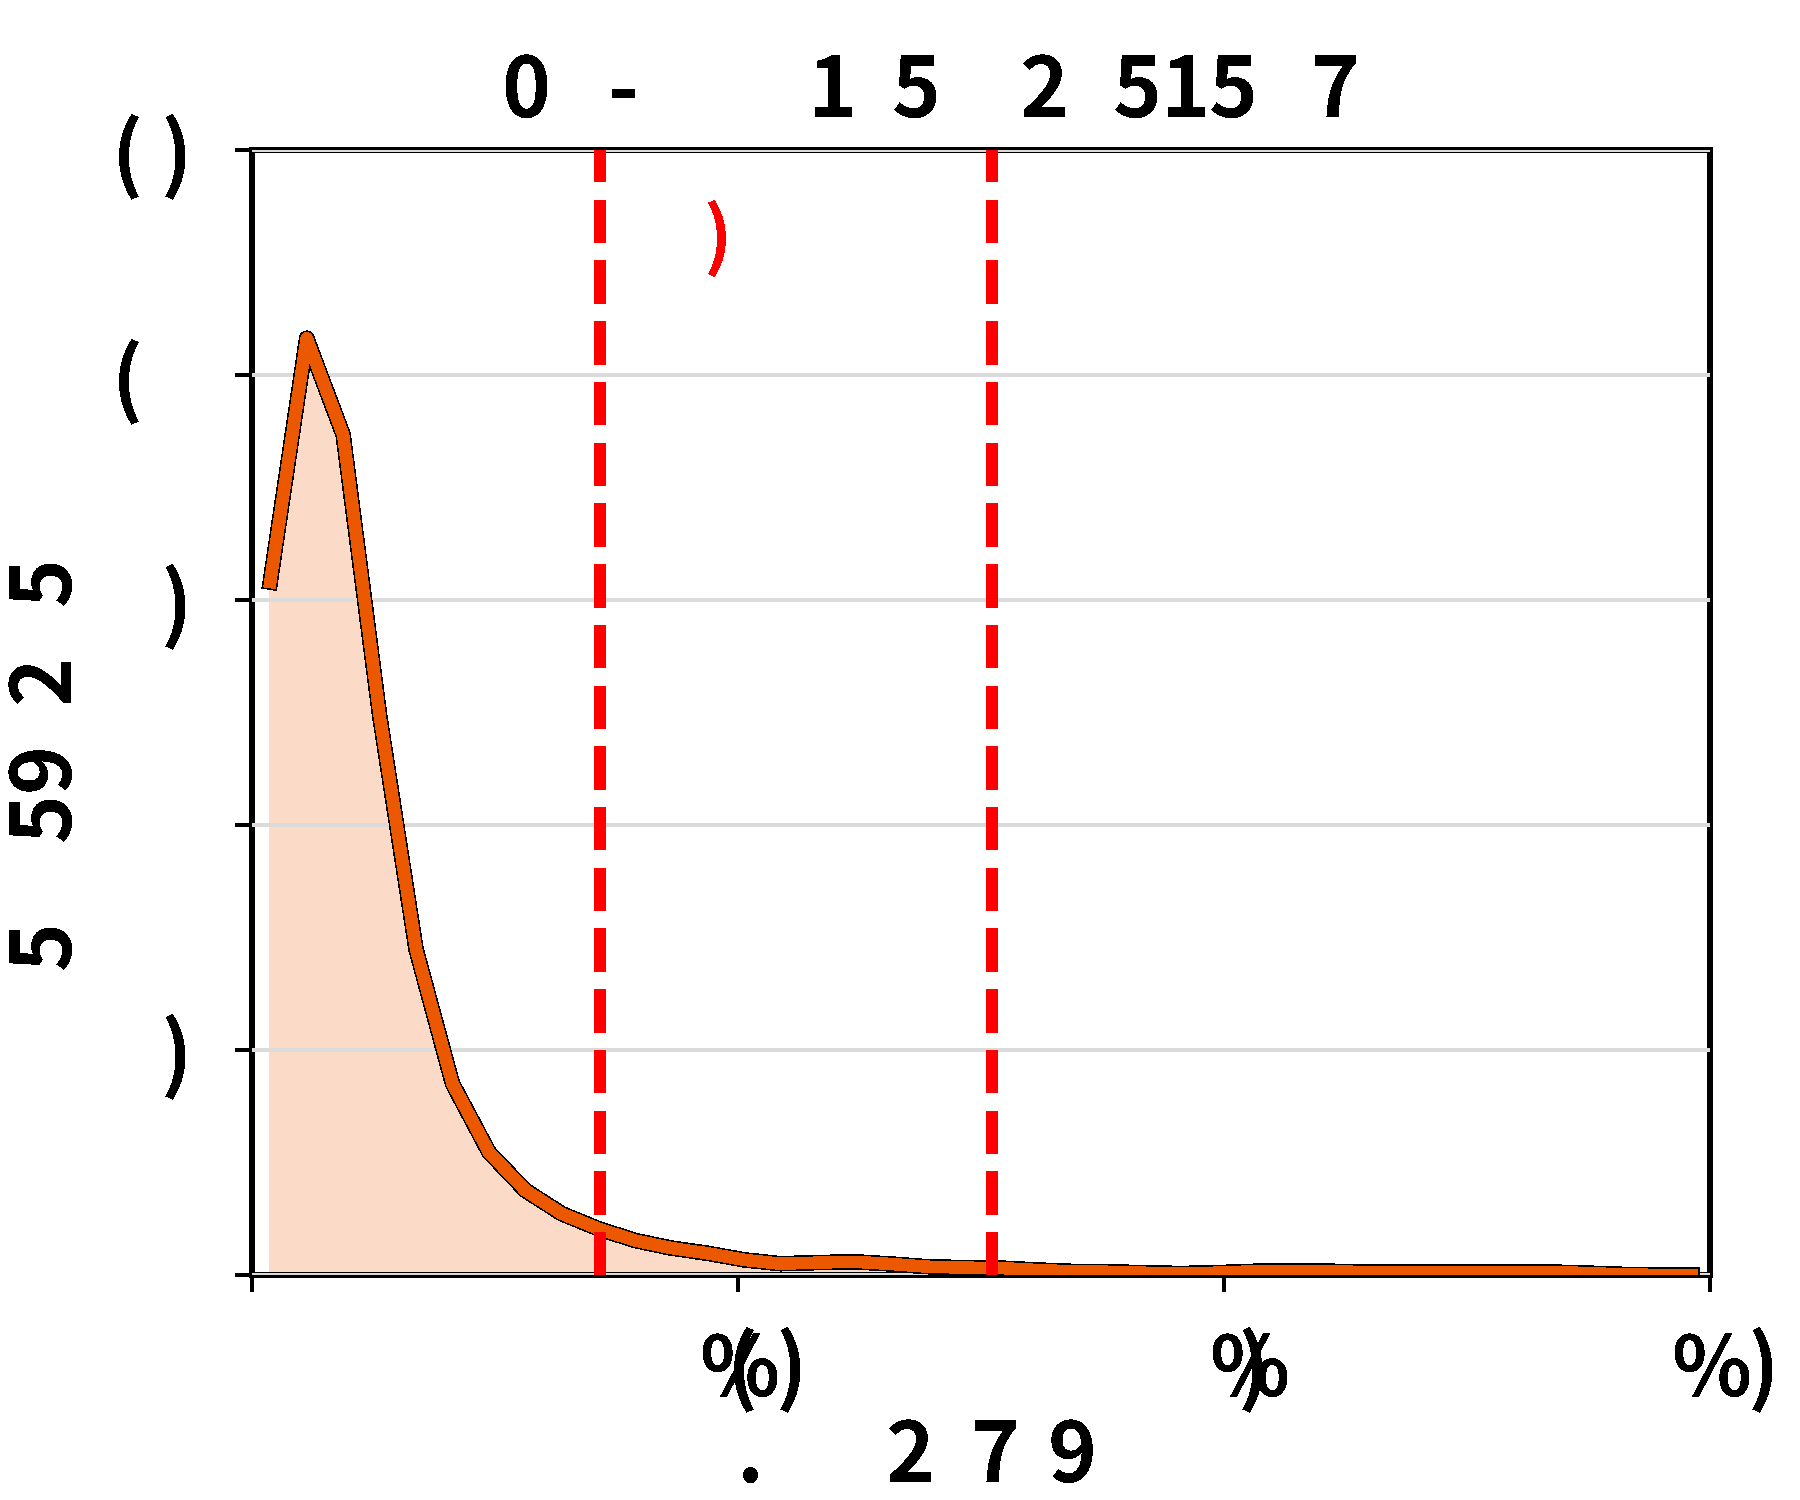
\includegraphics[width=0.8\linewidth]{Figures/appendix_figs/sab_str_replace_editor_duration_dist.pdf} % (f) optional
    \label{fig:sab_str_replace_editor}
  \end{subfigure}\hfill
  \begin{subfigure}[t]{0.32\textwidth}
    \centering
    % empty slot (keep layout)
    \label{fig:empty_slot_right}
  \end{subfigure}

  \caption{\textbf{工具执行时间分布。}工具执行时间表现出高度可变性并且难以预测。}

  \label{fig:tool_time}
\end{figure*}

\newpage
\section{KV 缓存命中率统计及解读}
\label{sec:kv_hit_rate_stats}

在我们的成本分解方程中~(\ref{eq:cost_decomp}），智能体服务的吞吐量损失主要来自于 \emph{非生产性的} 间接费用：
外部工具执行期间由抖动和空闲 KV 缓存引起的 KV 重新计算，即
$\text{Cost}_{\text{recompute}}$ 和 $\text{Cost}_{\text{caching}}$。当工具调用较短且可预测时，作用阶段仅占用 KV 很短的时间，因此 $\text{Cost}_{\text{caching}}$ 很小；因此，避免抖动占主导地位：较高的 KV 缓存命中率通常意味着更少的重新预填充和更高的吞吐量。

然而，当工具执行时间变化很大时（参见附录~\ref{app:tool_var}），基于 TTL 的调度器最终可能会为长工具调用固定 KV。
虽然这可以减少 $\text{Cost}_{\text{recompute}}$ 并提高 KV 缓存命中率，但同时会膨胀 $\text{Cost}_{\text{caching}}$ 并降低吞吐量。这有助于解释为什么 Continuum~\cite{li2025continuumefficientrobustmultiturn} 尽管实现了更高的 KV 缓存命中率，却仍可能在工具繁重的工作负载上表现不佳（图~\ref{fig:eval_infer_result},~\ref{fig:kv_hit_rate_data_statistics}）。

\noindent\textbf{ThunderAgent 通过显式平衡缓存和重新计算来适应这些制度。}
ThunderAgent 在第~\ref{sec:scheduling_policy} 节中为执行阶段程序引入时间衰减函数 $f(t)$，用于权衡
$\text{Cost}_{\text{caching}}$ 和 $\text{Cost}_{\text{recompute}}$；我们在附录~\ref{app:ft_discussion} 中严格推导了 \(f(t)\) 的最优函数形式。
通过逐步降低长时间空闲执行程序的有效显存优先级，调度器会驱逐它们的 KV 缓存，从而在控制重新计算的同时减少空闲缓存成本，并在实践中带来更高吞吐量（图~\ref{fig:eval_infer_result}）。







\newpage
\section{扩展的理论分析。}

\subsection{用于周期性抖动检测的时间衰减函数证明。}
\label{app:ft_discussion}


\begin{hypothesis}[Unpredictable Tool Execution Time]
\label{hyp:unpredictable_tool}
对于执行程序，我们假设调度器无法可靠地预测给定程序的工具返回时间（参见附录~\ref{app:tool_var}）。因此，衰减函数 $f$ 应该只以时间均匀的方式依赖已经经过的执行时间 $t$~\cite{parzen1999stochastic}.
\end{hypothesis}


\begin{hypothesis}[Boundary Conditions]
\label{hyp:boundary_conditions}
我们假设时间衰减函数 $f:[0,\infty)\rightarrow(0,1]$ 满足
\begin{equation}
f(0) = 1, \lim_{t\to\infty} f(t) = 0,
\label{eq:boundary_f}
\end{equation}
这些边界条件的直观解释是，当工具执行时间为 $0$，对应于没有工具调用的多轮交互，所有的智能体程序都简化为推理程序，因此 $f(t)=1$。相反，如果工具执行时间是无限的，智能体工作流就会崩溃为单轮生成，类似于标准聊天机器人服务，因为请求永远不会返回下一轮交互。在此制度下，设置 $f(t)=0$ 将衰减函数与请求级调度策略保持一致。
\end{hypothesis}

\begin{theorem}[Admissible Time Decay Functions]
\label{thm:admissible_decay}
假设下~\ref{hyp:unpredictable_tool} 和 \ref{hyp:boundary_conditions}，允许的时间衰减函数 $f$ 方程中的容量检查函数~\ref{eq:time_decay} 必须采用以下形式之一：连续时间的指数， $f(t)=e^{-\lambda t}$ 和 $\lambda>0$，或离散滴答时间的几何， $f(k)=x^{-k}$ 和 $x>1$.
\end{theorem}

\begin{proof}
我们通过首先形式化隐含的时间齐次性质来证明这个定理
假设~\ref{hyp:unpredictable_tool}。接下来，我们引入允许的时间衰减函数 $f$ 在边界条件下
假设~\ref{hyp:boundary_conditions}.
\smallskip

\noindent\textbf{不可预测的工具时间的形式化。} 让 $t$ 表示经过的作用时间，以挂钟时间（连续时间）或周期监视器滴答声（离散时间）测量。假设下~\ref{hyp:unpredictable_tool}，等待额外持续时间后的相对衰减 $\Delta$ 不应取决于绝对经过的时间 $t$，但仅限于增量 $\Delta$。我们将其形式化为函数的存在 $\phi:[0,\infty)\to(0,1]$ 这样，对于所有 $t,\Delta\ge 0$, \begin{equation} f(t+\Delta)=f(t)\,\phi(\Delta). \label{eq:time_homogeneous} \end{equation}

\noindent\textbf{半群方程。} 环境 $t=0$ 在方程中~\ref{eq:time_homogeneous} 并使用边界条件 $f(0)=1$
（来自假设~\ref{hyp:boundary_conditions}) 产量
$\phi(\Delta)=f(\Delta)$。代入回去，我们得到乘法
半群方程
\begin{equation}
f(t+\Delta)=f(t)\,f(\Delta),\qquad \forall t,\Delta\ge 0.
\label{eq:semigroup}
\end{equation}

\noindent \textbf{连续时间情况（指数衰减）。} 我们首先考虑连续时间的情况。
定义 $h(t)\triangleq \ln f(t)$。两边取对数
方程~\ref{eq:semigroup} 产生 \emph{柯西函数方程}
\begin{equation}
h(t+\Delta)=h(t)+h(\Delta).
\label{eq:cauchy}
\end{equation}
自从 $f(t)\in(0,1]$，我们有 $h(t)\le 0$ 为所有人 $t\ge 0$，这意味着
那 $h$ 上界为 $[0,\infty)$。在这种有界条件下，柯西函数方程只允许线性解
形式的 $h(t)=ct$ 对于某些人来说 $c\in\mathbb{R}$。写作 $\lambda\triangleq -c\ge 0$,
我们得到
\begin{equation}
f(t)=e^{-\lambda t}.
\label{eq:exp_decay}
\end{equation}
最后，边界条件 $\lim_{t\to\infty} f(t)=0$
（假设~\ref{hyp:boundary_conditions}) 排除 $\lambda=0$,
因此 $\lambda>0$.

\smallskip
\noindent \textbf{离散时间情况（几何衰减）。} 接下来我们考虑离散时间设置，其中经过的作用时间是
以整数刻度测量 $k\in\mathbb{Z}_{\ge 0}$.
方程~\ref{eq:semigroup} 变成
\begin{equation}
f(m+n)=f(m)\,f(n),\qquad \forall m,n\in\mathbb{Z}_{\ge 0}.
\label{eq:semigroup_discrete}
\end{equation}
环境 $n=1$ 产生递归 $f(k)=f(k-1)f(1)$。让 $\gamma \triangleq f(1)$，我们有
$f(k)=f(1)^k\triangleq \gamma^k$.
边界条件 $\lim_{k\to\infty} f(k)=0$ 意味着 $0<\gamma<1$.
等价地，我们可以参数化
\begin{equation}
f(k)=x^{-k},\qquad x\triangleq \gamma^{-1}>1.
\label{eq:geom_decay}
\end{equation}

\noindent 这样就完成了证明。
\end{proof}

\subsection{重新计算STP成本的证明}
\label{app:prefill_stpcost}
正如定义在 \autoref{sec:utility_model}，STP 重新计算成本由下式给出：
\begin{equation}
    \text{Cost}_{\text{recompute}} = \int_{0}^{t_{recompute}} c_i(t) \, dt
\end{equation}
在哪里 $c_i(t)$ 表示瞬时成本，与解码步骤成正比（即 $c_i(t) \propto t$）。出现这种比例的原因是分块预填充每次迭代处理恒定数量的 KV 对，从而导致累积计算随着时间的推移线性增加。因此，评估积分收益率 $\text{Cost}_{\text{recompute}} \propto t_{\text{recompute}}^2$。鉴于关系 $t_{\text{recompute}} = c_i \times T_{\text{decode}} / \text{chunk}$，其中两者 $T_{\text{decode}}$ 并且块大小是恒定的，因此：
\begin{equation*}
Cost_{\text{recompute}} \propto c_{i}^2
\end{equation*}

\subsection{最小化重新计算 STP 成本的证明}

\label{app:_minimized_STP_cost}
我们使用以下方法为最短优先驱逐策略的最优性提供了严格的证明： \textbf{交换论点}.

\textbf{问题定义。}
我们的目标是选择暂停程序的子集 $S$ 驱逐使得总回收内存满足 $\sum_{i \in S} c_i \ge \Delta C$，同时最小化总重新计算成本 $J(S) = \sum_{i \in S} c_i^2$。注意成本函数 $f(x) = x^2$ 是严格凸且超可加的（即 $(a+b)^2 > a^2 + b^2$ 为积极的 $a, b$).

\textbf{定理。}
最小化的最优策略 $J(S)$ 就是严格选择上下文长度最小的程序 $c_i$.

\textbf{证明。}
为了矛盾起见，假设最优集 $S^*$ 是 \textit{不是} 最短的程序集。这意味着存在一个“长”程序 $p_{long} \in S^*$ 和一个“短”节目 $p_{short} \notin S^*$ （可用但未选择）使得 $c_{short} < c_{long}$。

我们可以构造一个新集合 $S'$ 通过交换或分解 $p_{long}$。自从 $c_{long} > c_{short}$，我们可以概念化 $p_{long}$ 由一段长度组成 $c_{short}$ 和残留物 $r = c_{long} - c_{short}$.

替换选择 $p_{long}$ 和 $p_{short}$ （理论上剩余 $r$）改变成本。考虑由平方函数的凸性导出的不等式：
\begin{equation}
    c_{long}^2 = (c_{short} + r)^2 = c_{short}^2 + r^2 + 2 c_{short} r
\end{equation}
自从 $c_{short} > 0$ 和 $r > 0$, 交叉项 $2 c_{short} r > 0$。所以：
\begin{equation}
    c_{short}^2 + r^2 < c_{long}^2
\end{equation}

这种不平等意味着打破一个大的驱逐目标（$c_{long}$）分解为更小的组件（$c_{short} + r$) 严格减少平方和。
在我们的调度器的上下文中，这意味着如果我们满足内存约束 $\Delta C$ 使用大型程序，我们可以通过将其替换为总容量相同的可用较小程序（或其组合）来严格减少惩罚。

通过迭代地应用这种交换——用较小的未选择的程序替换最大的选定程序——我们单调地降低成本函数 $J(S)$。仅当不可能进行此类交换时，即当 $S$ 完全由具有最小可用上下文长度的程序组成。

\textbf{结论。}
最短优先策略是全局最优的，因为注意力的超线性成本（$O(L^2)$）对碎片的惩罚小于对聚合的惩罚。

\newpage
\section{端到端延迟分析}
\label{app:e2e}
尽管我们已在 \autoref{sec:intro} 中说明，对于自主智能体和智能体 RL rollout，程序级延迟（生成整个工作流所用时间）比每步端到端延迟更重要，这里仍比较 \ouralg、vLLM 和 Continuum 的平均每步延迟。\autoref{fig:e2e} 表明，在单个 H100 上以低或高并行工作流数量运行 GLM-4.6 和 Qwen3 235B，并搭配 mini-SWEAgent 与 OpenHands 时，\ouralg 显著优于 vLLM 和 Continuum。\textbf{Continuum 看似通过切换执行阶段程序改善了端到端延迟，但实际上会触发严重 KV 缓存抖动，从而推迟所有运行中程序的完成。}




\begin{figure*}[]
  \centering
  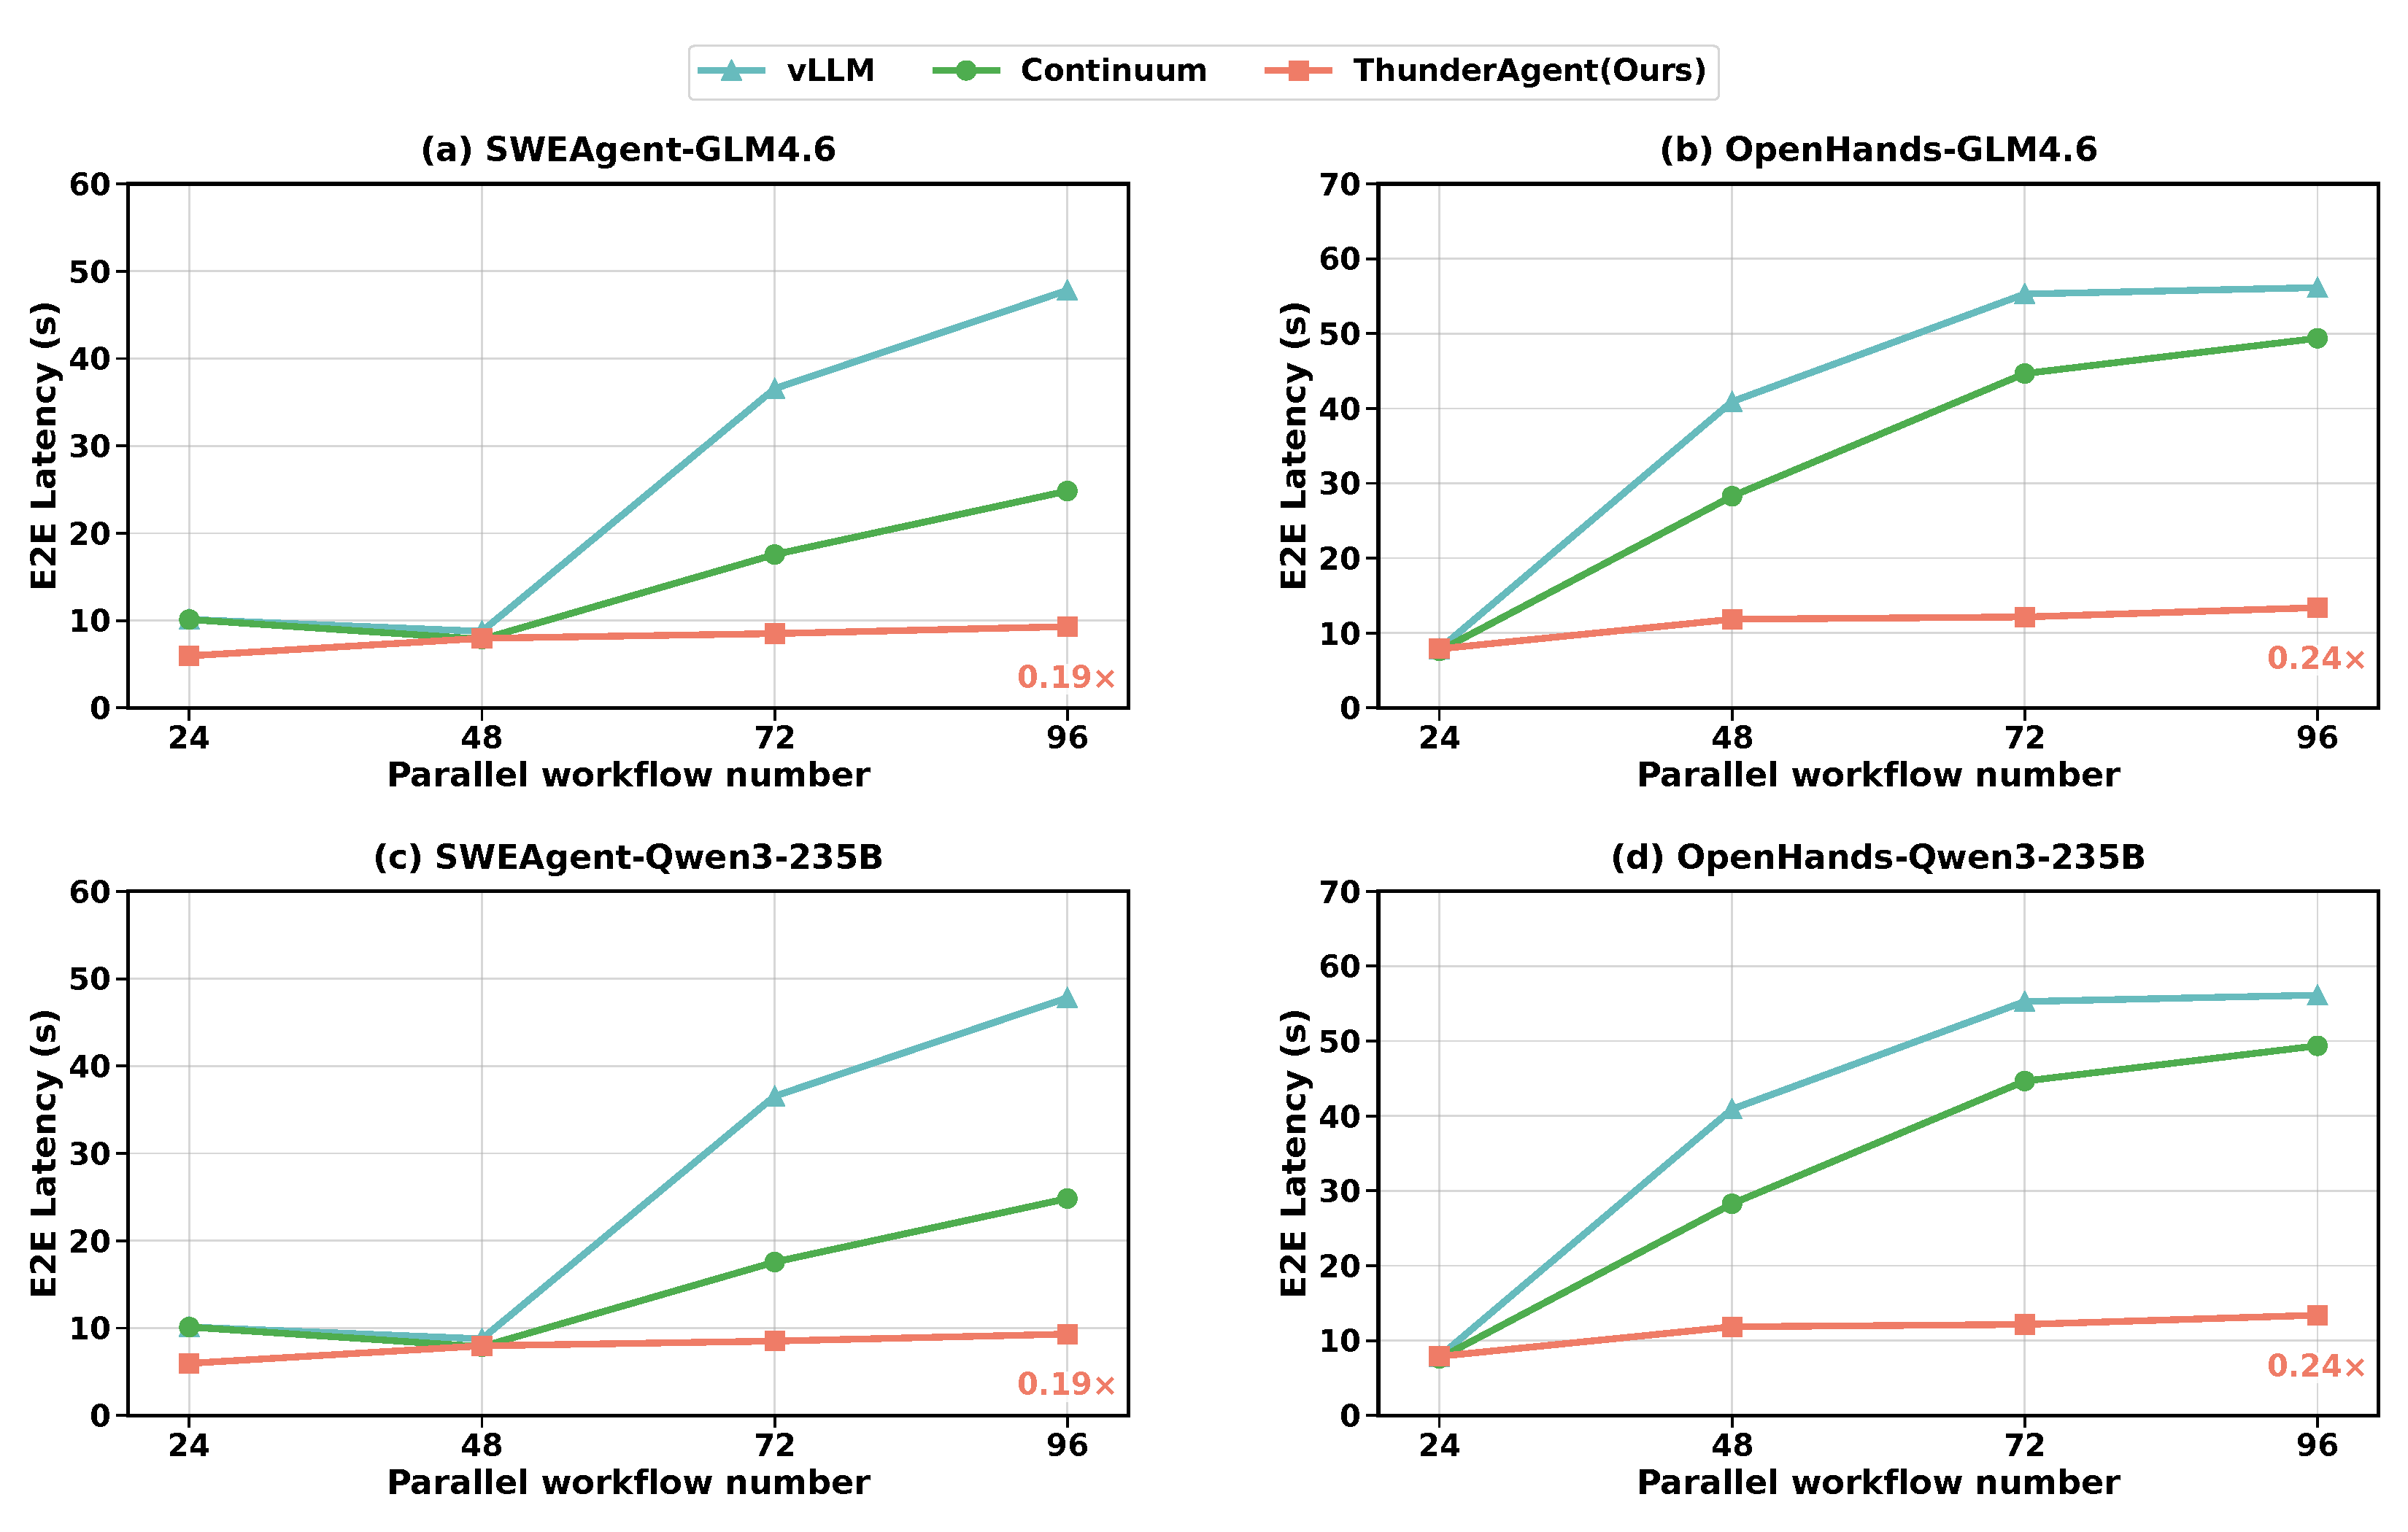
\includegraphics[width=0.7\textwidth]{Figures/latency_analysis_v4_final.pdf}
  \caption{端到端延迟比较}
  \label{fig:e2e}
\end{figure*}
% \begin{figure*}[!t]
%     \centering
%     \includegraphics[width=0.7·\columnwidth]{Figures/figure4_latency_reproduction.pdf}
%     \vspace{-2mm}
%     \caption{End-to-End latency comparision}
%     \label{fig:e2e}
% \vspace{-5mm}
% \end{figure*}

% You can have as much text here as you want. The main body must be at most $8$
% pages long. For the final version, one more page can be added. If you want, you
% can use an appendix like this one.

% The $\mathtt{\backslash onecolumn}$ command above can be kept in place if you
% prefer a one-column appendix, or can be removed if you prefer a two-column
% appendix.  Apart from this possible change, the style (font size, spacing,
% margins, page numbering, etc.) should be kept the same as the main body.
%%%%%%%%%%%%%%%%%%%%%%%%%%%%%%%%%%%%%%%%%%%%%%%%%%%%%%%%%%%%%%%%%%%%%%%%%%%%%%%
%%%%%%%%%%%%%%%%%%%%%%%%%%%%%%%%%%%%%%%%%%%%%%%%%%%%%%%%%%%%%%%%%%%%%%%%%%%%%%%
